%!TeX root=Memory.tex


\chapter{Disseny}
\label{ch:disseny}

Aquest capítol presenta el disseny tècnic i d'interacció de DemoChain.
Es descriu primer l'arquitectura global seguint el model C4 (context, contenidors i components), després el patró de
desplegament basat en Docker, tot seguit el disseny de la interfície web amb què interactua el votant, i finalment els
fluxos de comunicació principals representats com a diagrames de seqüència.


\section{Arquitectura: visió C4}
\label{sec:arquitectura:-visio-c4}

Per descriure l'arquitectura s'ha seguit el model C4 de Simon Brown, que ofereix quatre nivells de detall progressius.
En aquest capítol s'inclouen els tres primers nivells i el quart queda implicit al codi de l'aplicació.
Cada nivell s'orienta a un públic diferent: el primer dona una vista de conjunt útil per a qualsevol part interessada,
el segon situa les peces de \textit{software} que cal mantenir, i el tercer entra al detall dels components que
conviuen dins cada contenidor.

\subsection{Nivell 1 - Context}
\label{subsec:nivell-1--context}

El primer nivell mostra el sistema des de fora i n'identifica els actors humans i els sistemes externs amb què
interacciona (\autoref{fig:c4-c1}).
Hi ha dos rols humans diferenciats: el \textbf{Votant}, que proposa, vota eleccions des de la interfície web o inclus
gestiona organitzacions, i l'\textbf{Administrador} de nodes, que gestiona la llista blanca d'adreces autoritzades a
publicar \textit{hash}es a Ethereum.
El sistema en si interactua amb dues xarxes (Algorand i Ethereum) i amb una cartera externa que custodia les claus
privades del votant.

\begin{figure}[ht]
    \centering
    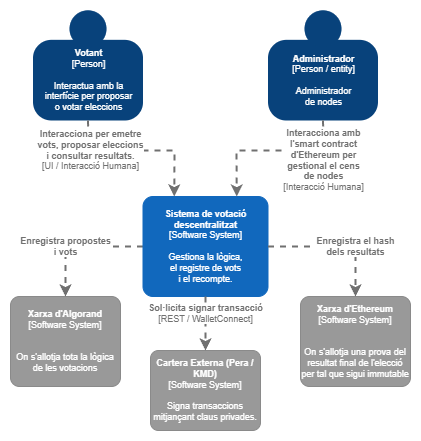
\includegraphics[width=0.85\textwidth]{chapters/images/disseny/c4/c1-context}
    \caption{Diagrama C4 de nivell 1: context de DemoChain.}
    \label{fig:c4-c1}
\end{figure}

La decisió de mantenir aquestes dues xarxes diferenciades es justifica al capítol d'Anàlisi: Algorand allotja la lògica
de votació en una xarxa permissionada de baix cost, i Ethereum actua únicament com a notari públic per a la prova final,
sense participar en cap pas intermedi del recompte.

\subsection{Nivell 2 - Contenidors}
\label{subsec:nivell-2-contenidors}

El segon nivell descompon el sistema en quatre contenidors de \textit{software}, cadascun amb una tecnologia i una
responsabilitat clares (\autopageref{fig:c4-c2}):

\begin{itemize}
    \item \textbf{Client - Interfície web} (React).
    Punt d'entrada de l'usuari.
    Construeix transaccions \ac{ABI}, demana signatures a la cartera, consulta l'estat de la cadena i hi escriu
    propostes, vots i operacions de gestió d'organitzacions (si es el cas).

    \item \textbf{Contracte intel·ligent d'Algorand} (Algopy/TEAL).
    Conté la lògica de propostes, eleccions i organitzacions.
    Manté l'estat persistent (cens, paperetes, finestres temporals) a Box Storage.

    \item \textbf{Servei d'ancoratge} (Python).
    Procés autònom que s'executa paral·lelament a cada node.
    Detecta eleccions tancades, en deriva un \textit{hash} determinista i l'envia al contracte d'Ethereum.

    \item \textbf{Contracte intel·ligent d'Ethereum} (Solidity).
    El \textit{NotaryContract}: acumula els \textit{hash}es enviats pels nodes i registra l'elecció com a ancorada quan
    se n'arriba al consens de \textit{K-of-N}.
\end{itemize}

\begin{figure}[ht]
    \centering
    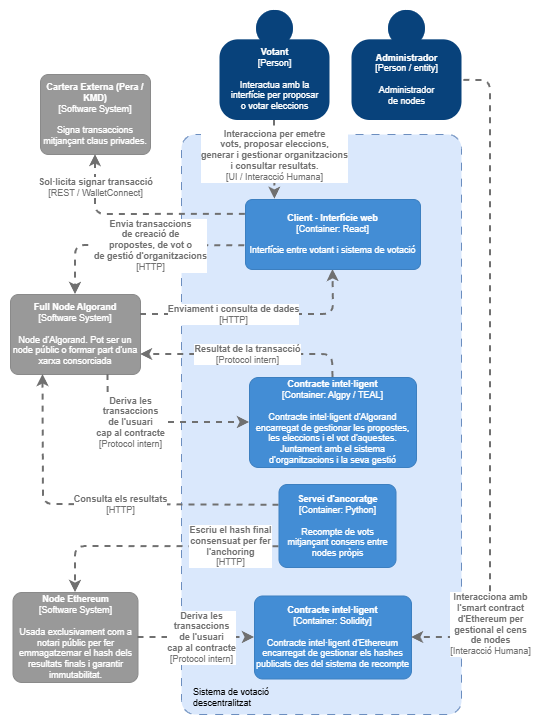
\includegraphics[width=0.9\textwidth]{chapters/images/disseny/c4/c2-containers}
    \caption{Diagrama C4 de nivell 2: contenidors de DemoChain.}
    \label{fig:c4-c2}
\end{figure}

El client no parla directament amb el contracte: tota interacció passa per un \textbf{Full Node Algorand}, que actua de
gateway HTTP cap a la xarxa.
Aquesta separació permet que diferents universitats puguin oferir el seu propi node sense haver de tocar el client.
De manera anàloga, el servei d'ancoratge llegeix paperetes del node Algorand i escriu al \textit{NotaryContract} a
través d'un node Ethereum, però aquest últim queda fora del \textit{software} del projecte (s'utilitza un proveïdor de
la testnet d'Ethereum, Sepolia).

\subsection{Nivell 3 - Components}
\label{subsec:nivell-3---components}

El tercer nivell entra dins de cada contenidor i hi descompon els components funcionals.
Es presenten quatre vistes, una per contenidor.

\subsubsection{Client web}

El client és una aplicació de pàgina única (SPA) que organitza la responsabilitat en capes ben delimitades, de manera
que els canvis a la interfície no impacten la lògica de domini ni la integració amb la cadena.

\begin{figure}[ht]
    \centering
    
\includegraphics[width=\textwidth]{chapters/images/disseny/c4/c3-component-client}
    \caption{Components del client web.}
    \label{fig:c4-c3-client}
\end{figure}

Els components principals són:

\begin{itemize}
    \item \textbf{Router}, que gestiona les rutes i els \textit{loaders} de precàrrega de dades amb
    \texttt{react-router-dom}.

    \item \textbf{Page Views}, que controlen l'estat de cada pantalla i orquestren formularis amb
    \texttt{react-hook-form} i \texttt{zod}.

    \item \textbf{Theme \& Translation Providers}, basats en React Context i \texttt{i18next}, que mantenen el tema
    clar/fosc i les tres llengües suportades.

    \item \textbf{Data Cache \& Sync Manager} (\texttt{react-query}), que ofereix una caché coherent sobre les consultes
    a la cadena i facilita la invalidació després de cada transacció.

    \item \textbf{Algorand Queries \& Mutations}, conjunt de \textit{custom hooks} que encapsulen les operacions
    asíncrones del contracte.

    \item \textbf{UI Component Library}, els elements gràfics reutilitzables (\texttt{RankingList},
    \texttt{PairwiseGrid}, etc.) construïts amb TailwindCSS\@.

    \item \textbf{Wallet Connect \& Manager} (\texttt{use-wallet-react}), responsable de la sessió de cartera i de
    demanar signatures.

    \item \textbf{Smart Contract Client Wrapper}, que utilitza \texttt{algosdk} per generar transaccions \ac{ABI} a
    partir del descriptor \ac{ARC}56 del contracte.

    \item \textbf{Domain Logic Layer}, codi TypeScript pur que conté \textit{mappers}, validacions i el càlcul del
    mètode de Schulze.
\end{itemize}

El càlcul del guanyador amb Schulze viu al client perquè el contracte d'Algorand no emmagatzema cap resultat
precalculat: només paperetes individuals.
Això simplifica el contracte i permet que qualsevol persona pugui reproduir el recompte de manera independent.

\subsubsection{Contracte intel·ligent d'Algorand}

El contracte té com a punt d'entrada un \textbf{encaminador principal} que classifica cada transacció rebuda i la deriva
al mòdul adient.
Els mòduls coexisteixen al mateix \textit{application}, però estan separats lògicament per responsabilitats
(\autoref{fig:c4-c3-algorand}):

\begin{itemize}
    \item \textbf{Lògica de votació}: rep el vot, comprova que la direcció pertany al cens i que la proposta està en una
    finestra vàlida, i finalment emet o sobreescriu el vot.

    \item \textbf{Lògica de propostes}: rep i valida les propostes (dates, opcions, organització) i les desa a
    l'emmagatzematge.

    \item \textbf{Emmagatzematge d'estat}: utilitza Algorand Box Storage per persistir propostes, eleccions, vots
    d'aprovació, vots d'elecció, organitzacions i censos.
\end{itemize}

\begin{figure}[ht]
    \centering
    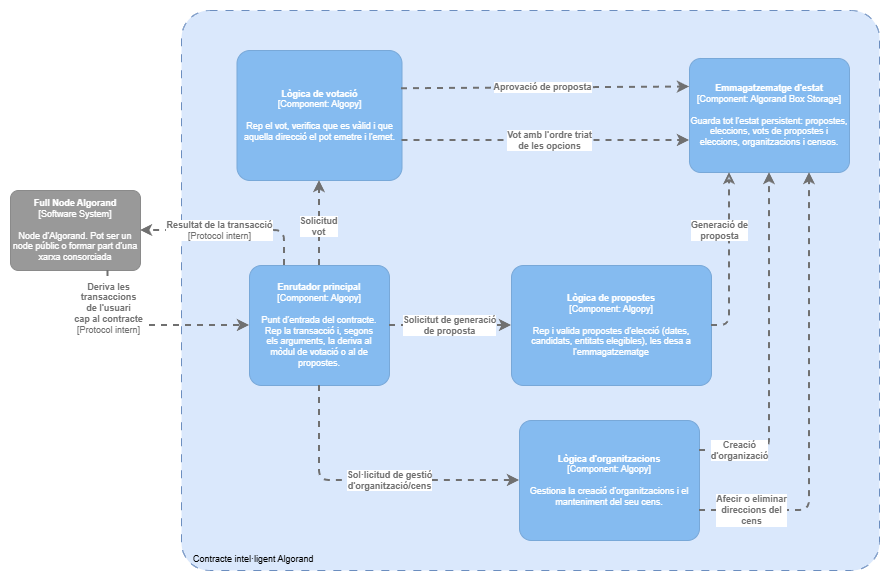
\includegraphics[width=\textwidth]{chapters/images/disseny/c4/c3-component-sc-algorand}
    \caption{Components del contracte intel·ligent d'Algorand.}
    \label{fig:c4-c3-algorand}
\end{figure}

\subsubsection{Servei d'ancoratge}

El servei d'ancoratge és un procés Python autònom dissenyat per executar-se paral·lelament a cada node
(\autoref{fig:c4-c3-anchoring}).
La seva responsabilitat és detectar quan una elecció es tanca, calcular-ne un \textit{hash} determinista i enviar-lo al
\textit{NotaryContract} d'Ethereum.

\begin{figure}[ht]
    \centering
    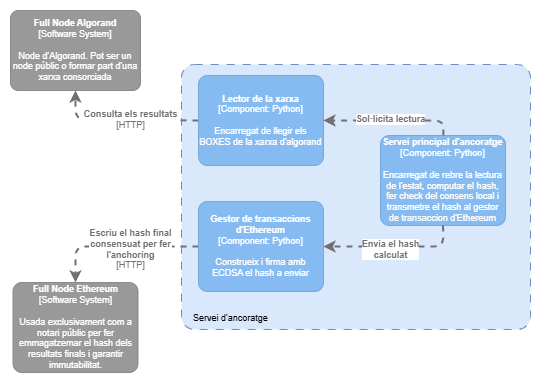
\includegraphics[width=\textwidth]{chapters/images/disseny/c4/c3-component-anchoring}
    \caption{Components del servei d'ancoratge.}
    \label{fig:c4-c3-anchoring}
\end{figure}

La clau d'aquest disseny és el determinisme: tots els nodes han de produir exactament el mateix \textit{hash} a partir
del mateix estat de la cadena.
Per garantir-ho, el servei ordena lexicogràficament les paperetes per direcció del votant i en genera una representació
\ac{JSON} canònica (claus ordenades, sense espais) abans d'aplicar \ac{SHA}-256.
Així s'evita que diferències accidentals d'ordre o format facin divergir nodes honestos.

\subsubsection{Contracte intel·ligent d'Ethereum}

El \textit{NotaryContract} (\autoref{fig:c4-c3-ethereum}) implementa el consens \textit{K-of-N} entre els nodes
universitaris autoritzats.
L'administrador manté una llista blanca de direccions Ethereum i, abans que comenci l'ancoratge d'una elecció, l'obre al
contracte.
En aquest moment es congelen tant la llista de nodes autoritzats com el llindar K (\textit{ceil}(2/3 N)), de manera que
altes o baixes posteriors no afecten les eleccions ja obertes.

\begin{figure}[ht]
    \centering
    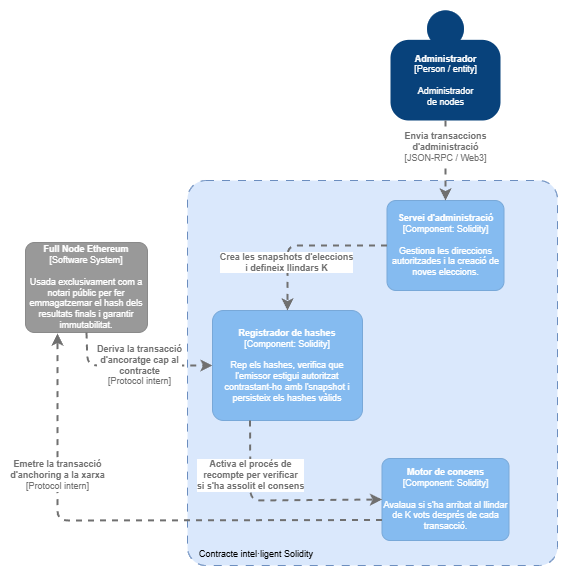
\includegraphics[width=\textwidth]{chapters/images/disseny/c4/c3-component-sc-ethereum}
    \caption{Components del contracte intel·ligent d'Ethereum.}
    \label{fig:c4-c3-ethereum}
\end{figure}

Cada node pot enviar un únic \textit{hash} per elecció.
Quan K nodes coincideixen en el mateix valor, el contracte emet un esdeveniment públic que registra l'elecció com a
ancorada de manera immutable.
La consulta posterior (quin \textit{hash} va enviar cada node, quan, i si finalment s'ha consensuat) és lliure i no
requereix cap autorització.


\section{Patró de desplegament}
\label{sec:patro-de-desplegament}

\subsection{Stack Docker Compose}
\label{subsec:stack-docker-compose}

Tot l'entorn local de DemoChain es desplega amb un únic fitxer \texttt{docker-compose.yml}.
Aquesta decisió persegueix tres objectius: (1) que qualsevol desenvolupador o universitat pugui aixecar el sistema amb
una sola comanda, (2) aïllar les versions concretes d'Algorand, l'\textit{indexer} i el client, i (3) reproduir en local
la mateixa topologia que s'espera en producció a cada node universitari.

La pila de serveis és la següent:

\begin{itemize}
    \item \textbf{algod}: el node d'Algorand.
    A dins conté dos nodes interns (un \textit{lead} a 8080 i un \textit{follower} a 8081) i el dimoni \ac{KMD} que
    custodia les claus de prova.

    \item \textbf{contract-deploy}: contenidor efímer basat en \texttt{uv} (Python 3.12) que compila el contracte amb
    PuyaPy i el desplega contra \texttt{algod}.

    \item \textbf{indexer-db}: una instància PostgreSQL que actua de magatzem per a l'\textit{indexer}.

    \item \textbf{conduit}: lector de \textit{state deltas} del \textit{follower} d'Algorand que alimenta la base de
    dades.

    \item \textbf{indexer}: l'\textit{indexer} d'Algorand, que ofereix una \ac{API} HTTP de cerca sobre la cadena.

    \item \textbf{client}: el contenidor del client web, basat en Bun, que serveix Vite en mode \textit{hot-reload}.
\end{itemize}

\subsection{Inicialització i flux \texttt{APP\_ID}}
\label{subsec:inicialitzacio-i-flux-texttt{app_id}}

Un punt rellevant del disseny és com s'enllaça el client amb el contracte desplegat.
El servei \texttt{contract-deploy} no és un servei de llarga durada: només existeix per construir el contracte,
desplegar-lo a \texttt{algod} i deixar el seu identificador disponible al client.
El flux és:

\begin{enumerate}
    \item \texttt{algod} arrenca i el \textit{healthcheck} confirma que respon.

    \item \texttt{contract-deploy} sincronitza les dependències amb \texttt{uv sync}, executa la \textit{build} del
    contracte i el desplega.

    \item De la sortida del desplegament n'extreu el valor \texttt{app\_id} i el persisteix com a \texttt{VITE\_APP\_ID}
    a \texttt{client/.env.local}.

    \item Només llavors el servei \texttt{client} arrenca, ja sabent contra quina aplicació ha d'apuntar.
\end{enumerate}

Quan es vol reiniciar la cadena (per exemple amb \texttt{docker compose down -v}), el cicle es repeteix i el client rep
automàticament el nou \texttt{APP\_ID}.
Així no cal cap intervenció manual per mantenir client i contracte sincronitzats.

\subsection{Aixecar un node d'Algorand}
\label{subsec:aixecar-un-node-d'algorand}

El mateix \texttt{docker-compose.yml} serveix de plantilla per desplegar un node real.
Cada entitat participant en el consorci aixeca la seva pròpia còpia del compose, però apuntant el seu \texttt{algod} a
la xarxa permissionada compartida i afegint-hi el servei d'ancoratge amb les seves credencials Ethereum.
El client web és estàtic i, per tant, qualsevol node pot servir-lo sense que això comprometi la integritat del sistema:
la confiança recau en el consens \textit{K-of-N} del \textit{NotaryContract}, no en la disponibilitat d'un node concret.


\section{Disseny de la interfície d'usuari}
\label{sec:disseny-de-la-interficie-d'usuari}

La interfície s'ha dissenyat amb un objectiu principal: que un votant que es connecti per primera vegada puguin entendre
què està a punt de fer i en quin punt del cicle es troba cada proposta, sense necessitat de conèixer els detalls de la
cadena.
Per aconseguir-ho s'han aplicat tres principis transversals:

\begin{itemize}
    \item \textbf{Vocabulari uniforme}.
    Els termes \textit{proposta}, \textit{elecció}, \textit{aprovació}, \textit{cens} i \textit{organització} es fan
    servir de manera consistent a totes les pantalles i corresponen al llenguatge ubic definit a l'anàlisi.

    \item \textbf{Múltiples idiomes i tema personalitzable}.
    La interfície està traduïda a català, castellà i anglès, i suporta tema clar i fosc.

    \item \textbf{Estat visible}.
    Cada proposta indica de manera explícita en quin estat del cicle es troba mitjançant \textit{badges} i filtres,
    evitant que el votant hagi d'inferir-ho a partir de dates.
\end{itemize}

\subsection{Llengües, tema i navegació global}
\label{subsec:llengues-tema-i-navegacio-global}

La pantalla d'inici presenta la proposta de valor del producte i serveix com a entrada al sistema.
La capçalera global, present a totes les rutes, ofereix accés directe a les seccions principals (\textit{Inici},
\textit{Organitzacions}, \textit{Propostes}, \textit{Nova proposta}), al selector d'idioma, al canvi de tema i al botó
de connexió de cartera (\autoref{fig:ui-landing}).

\begin{figure}[ht]
    \centering
    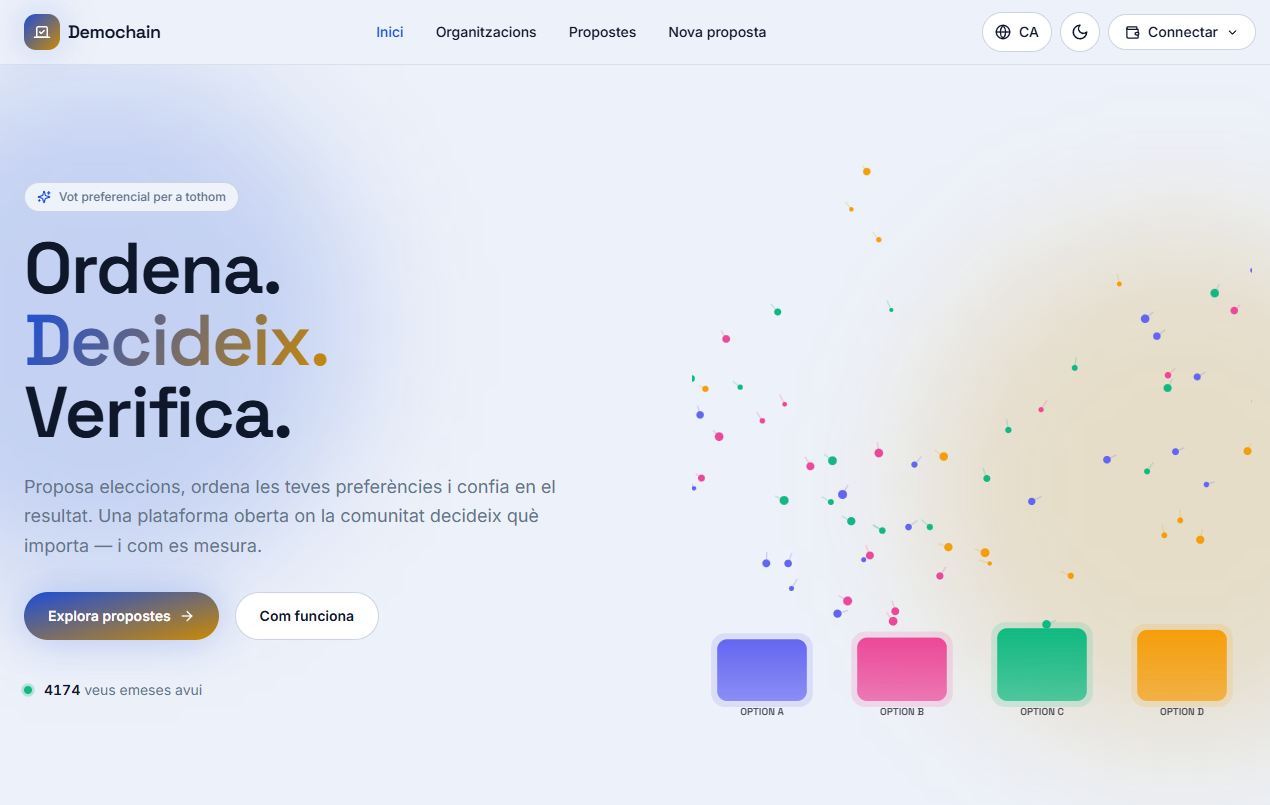
\includegraphics[width=\textwidth]{chapters/images/disseny/screenshots/01-landing}
    \caption{Pantalla d'inici de DemoChain. Capçalera de navegació, selector d'idioma i connexió de cartera.}
    \label{fig:ui-landing}
\end{figure}

\subsection{Gestió d'organitzacions}
\label{subsec:gestio-d'organitzacions2}

Les organitzacions són l'arrel de qualsevol activitat de votació: una proposta sempre pertany a una organització i només
els membres del seu cens hi poden participar.
La pantalla de llistat mostra les organitzacions a què pertany o que administra l'usuari connectat, amb una insígnia
d'\textit{Organitzador} quan és el cas (\autoref{fig:ui-organizations}).

\begin{figure}[ht]
    \centering
    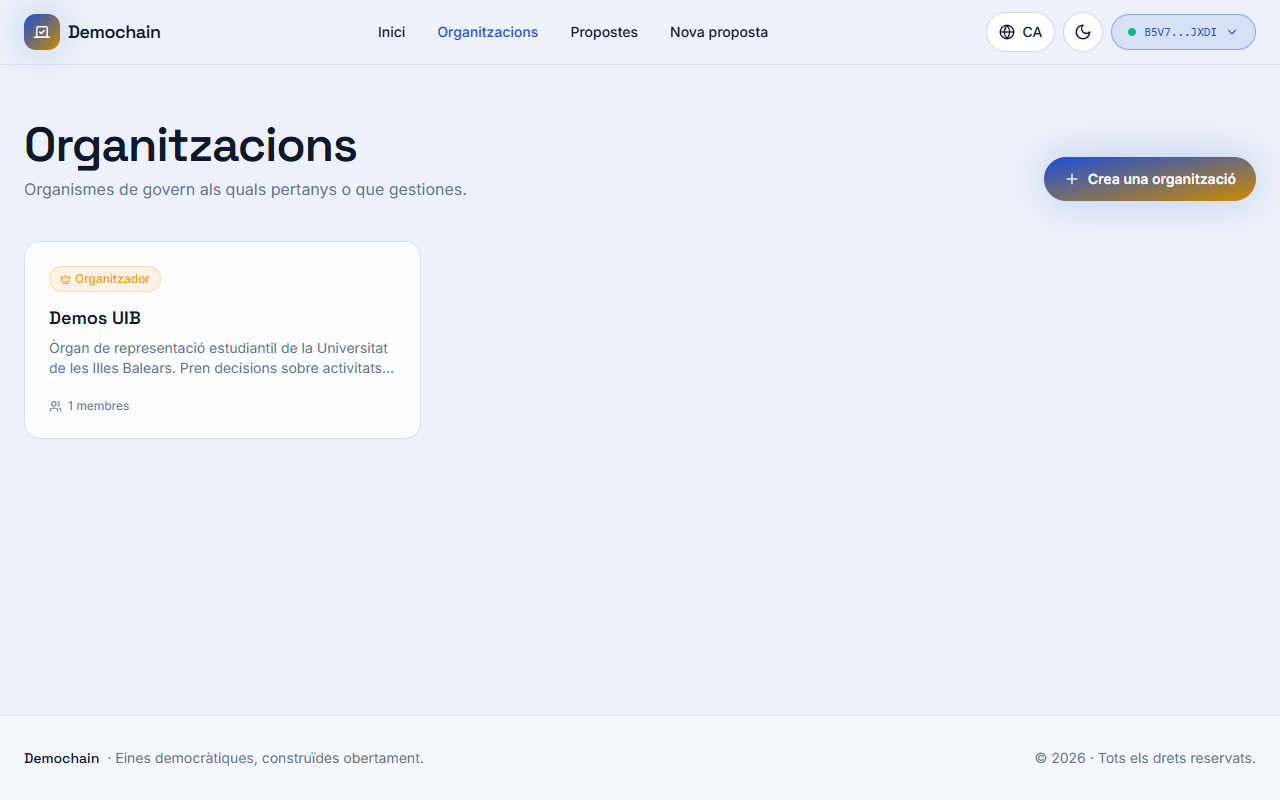
\includegraphics[width=\textwidth]{chapters/images/disseny/screenshots/02-organizations}
    \caption{Llistat d'organitzacions a què pertany el votant connectat.}
    \label{fig:ui-organizations}
\end{figure}

El detall d'una organització presenta dues pestanyes complementàries: \textbf{Propostes} (les propostes obertes o
tancades d'aquesta organització) i \textbf{Cens} (les adreces autoritzades a participar)
(\autoref{fig:ui-organization-detail}).
L'administrador pot afegir o eliminar membres des de la pestanya de cens, sigui d'un en un o per càrrega massiva
mitjançant un fitxer \ac{CSV}.
La interfície amaga al votant la complexitat de la transacció subjacent: el client trosseja internament les adreces en
lots compatibles amb el límit del contracte (set adreces per transacció) i guia el votant pel procés de signar les
transaccions consecutives.

\begin{figure}[ht]
    \centering
    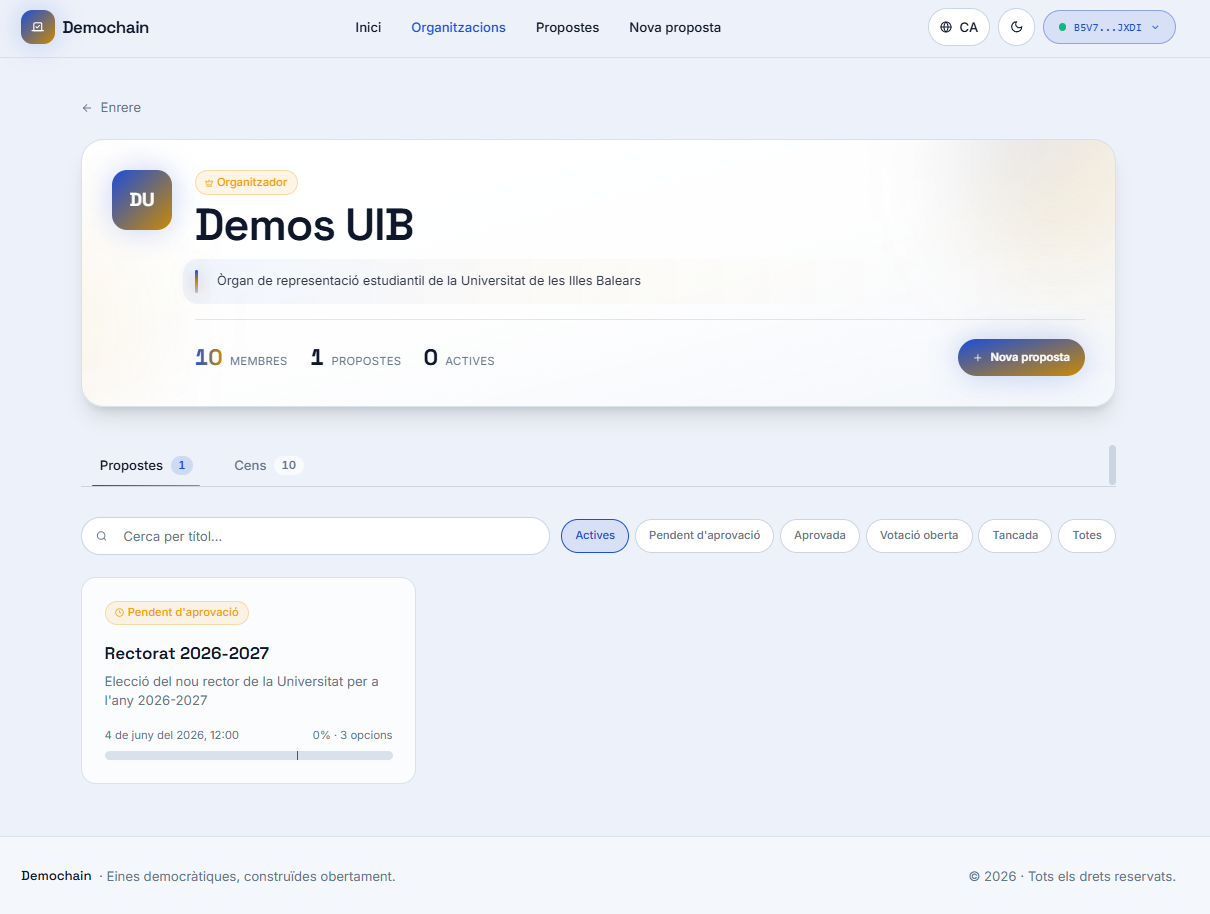
\includegraphics[width=\textwidth]{chapters/images/disseny/screenshots/03-organization-detail}
    \caption{Detall d'una organització, amb pestanyes de propostes i cens. L'organització té una proposta activa, encara sense vots d'aprovació.}
    \label{fig:ui-organization-detail}
\end{figure}

\subsection{Propostes i cicle de vida}
\label{subsec:propostes-i-cicle-de-vida}

La pantalla de propostes presenta totes les propostes visibles per a l'usuari, amb cercador i filtres per estat:
\textit{Actives}, \textit{Pendent d'aprovació}, \textit{Aprovada}, \textit{Votació oberta}, \textit{Tancada} i
\textit{Totes}.
Aquests estats segueixen exactament la màquina d'estats descrita a la documentació funcional del sistema
(\textit{PendingApproval}, \textit{PendingStart}, \textit{Open}, \textit{Closed}, \textit{Rejected}) i serveixen perquè
el votant detecti d'un cop d'ull en quines propostes pot actuar i en quines no (\autoref{fig:ui-proposals-list}).

\begin{figure}[ht]
    \centering
    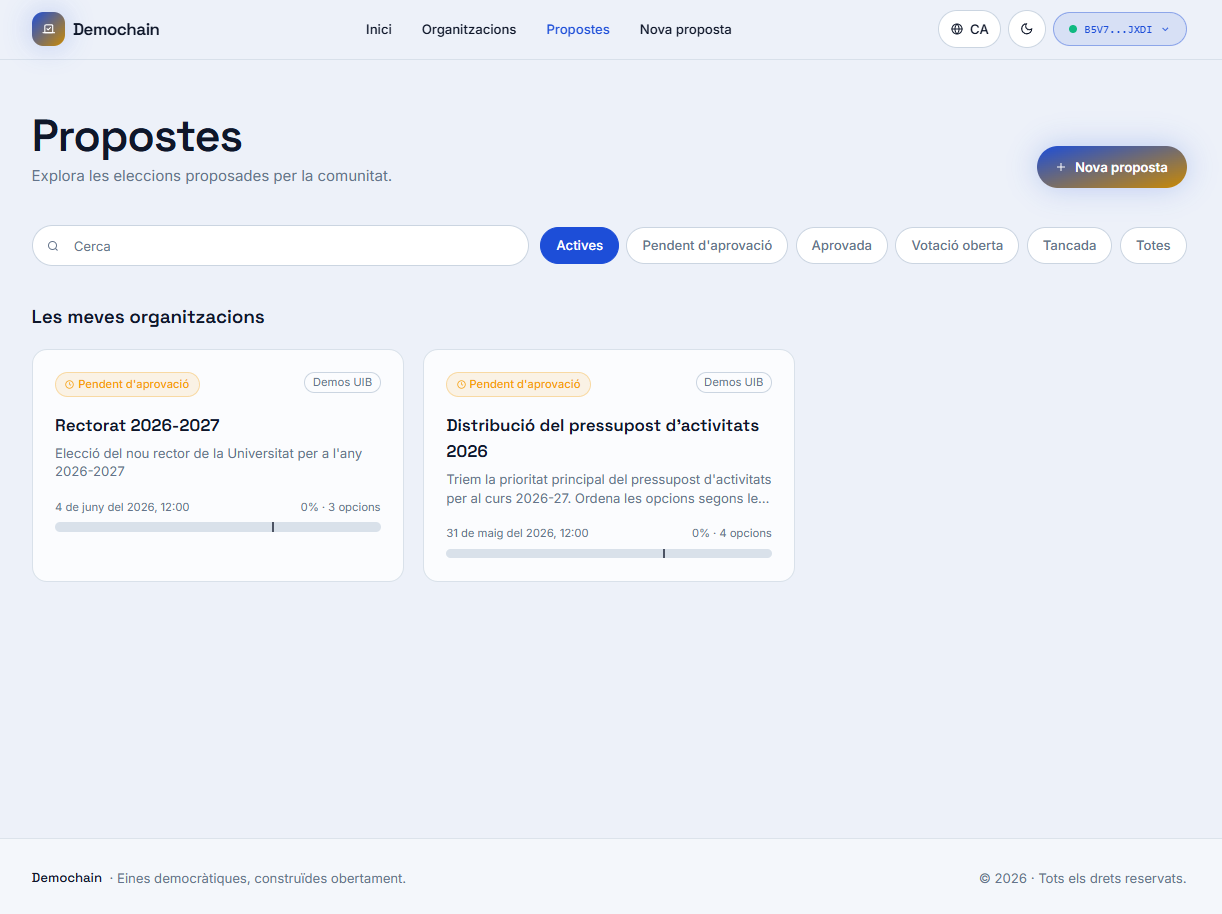
\includegraphics[width=\textwidth]{chapters/images/disseny/screenshots/04-proposals-list}
    \caption{Llistat de propostes amb filtres per estat. L'usuari que veu aquesta pantalla té dues propostes que estan \textit{pendents d'aprovació} de l'organització \textit{``Demos UIB''} (organització a la que pertany).}
    \label{fig:ui-proposals-list}
\end{figure}

\subsection{Creació d'una proposta}
\label{subsec:creacio-d'una-proposta}

La creació d'una proposta s'ha modelat com un assistent de cinc passos: \textit{Organització}
(\ref{fig:ui-new-proposal-1}), \textit{Bàsics} (\ref{fig:ui-new-proposal-2}), \textit{Dates}
(\ref{fig:ui-new-proposal-3}), \textit{Opcions} (\ref{fig:ui-new-proposal-4}) i \textit{Revisió}
(\ref{fig:ui-new-proposal-5}).
La divisió en passos persegueix dos objectius: dividir mentalment la decisió (cada pas demana un únic tipus
d'informació) i poder validar restriccions complexes -com la finestra temporal mínima- abans d'avançar al pas següent.
Tot el formulari es valida amb \texttt{zod}, de manera que cap dada arriba al contracte si no compleix les regles
bàsiques.
Una vegada es crea la proposta es reencamina a la pantalla per aprovar-la o revocar-la (\autoref{fig:ui-proposal}.
Quan la proposta s'aprova es veu tal com a la \autoref{fig:ui-proposal-aproved}).

\begin{figure}[ht]
    \centering
    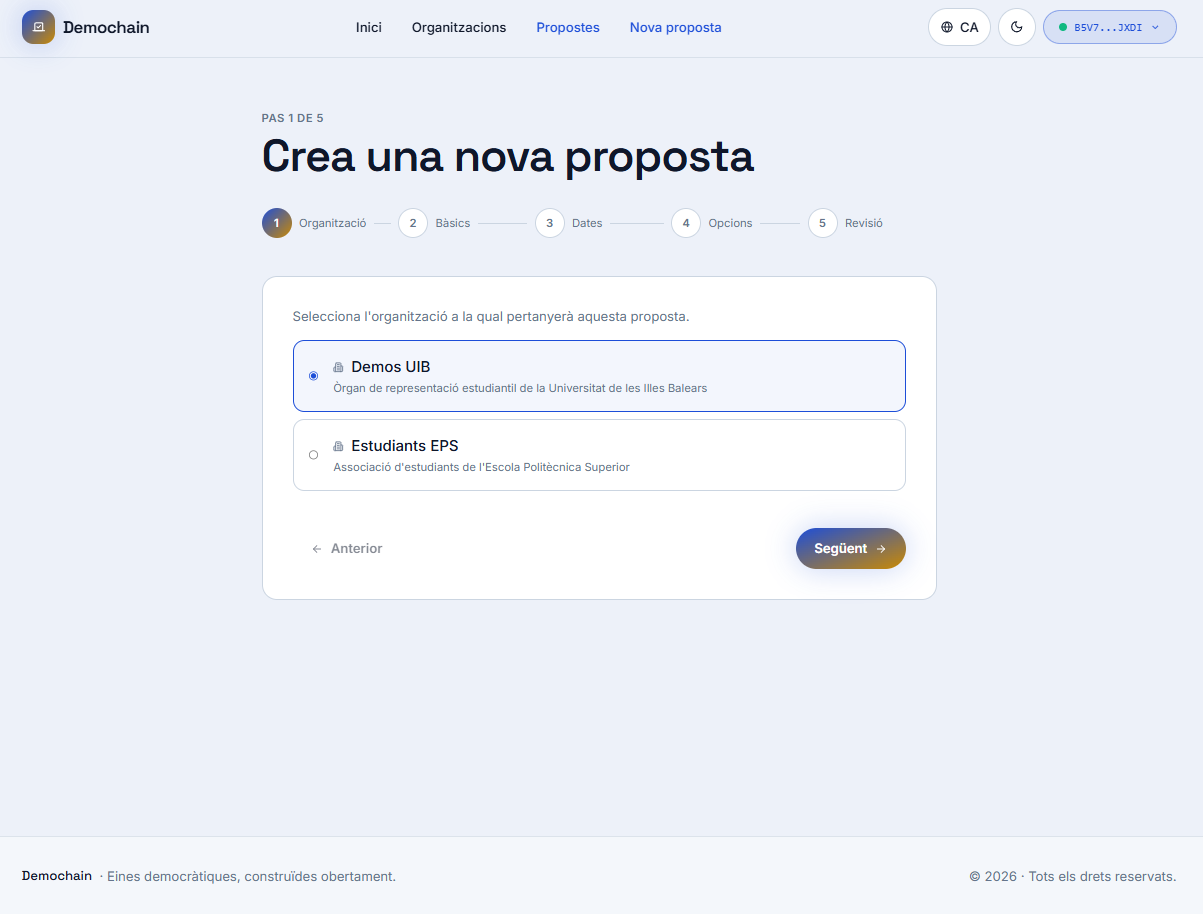
\includegraphics[width=\textwidth]{chapters/images/disseny/screenshots/05-new-proposal-1}
    \caption{Assistent de creació d'una proposta, pas \textit{Organització}.}
    \label{fig:ui-new-proposal-1}
\end{figure}

\begin{figure}[ht]
    \centering
    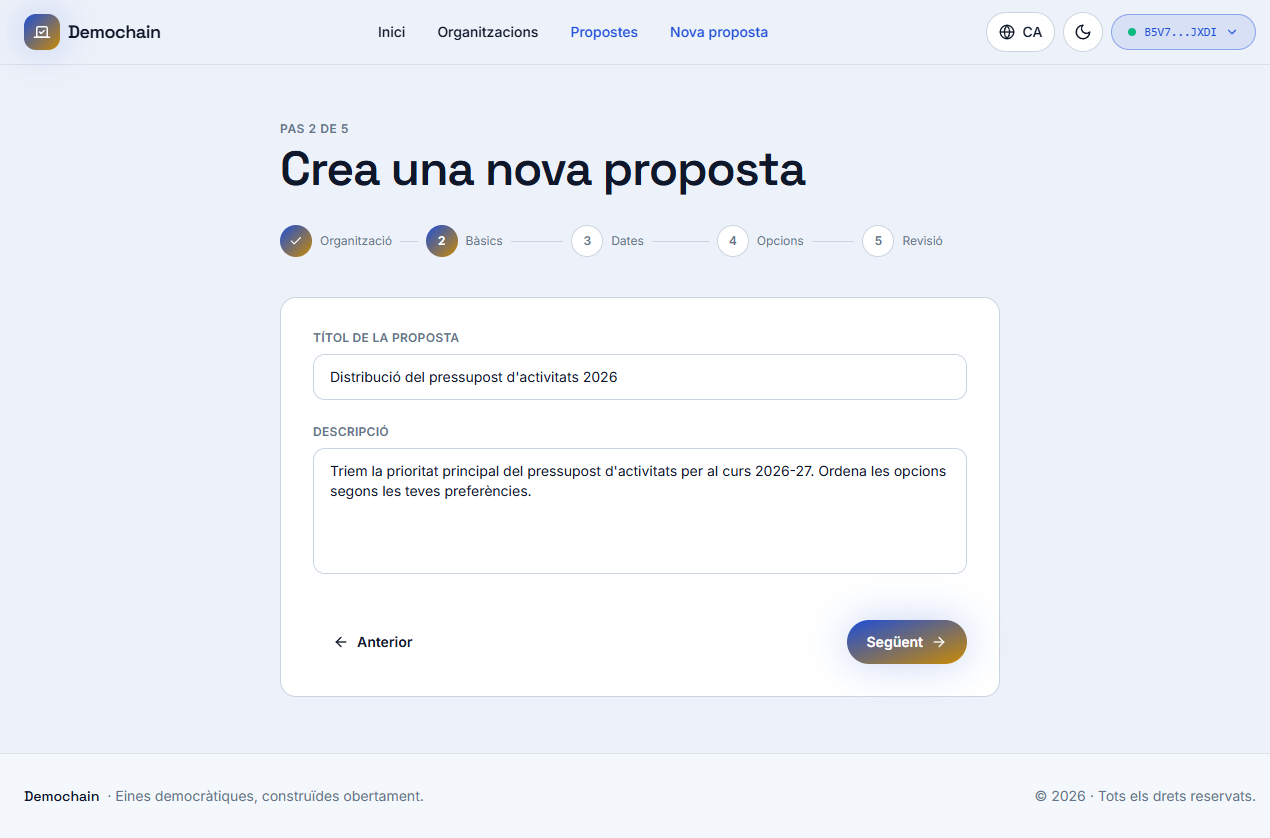
\includegraphics[width=\textwidth]{chapters/images/disseny/screenshots/05-new-proposal-2}
    \caption{Assistent de creació d'una proposta, pas \textit{Bàsics}.}
    \label{fig:ui-new-proposal-2}
\end{figure}

\begin{figure}[ht]
    \centering
    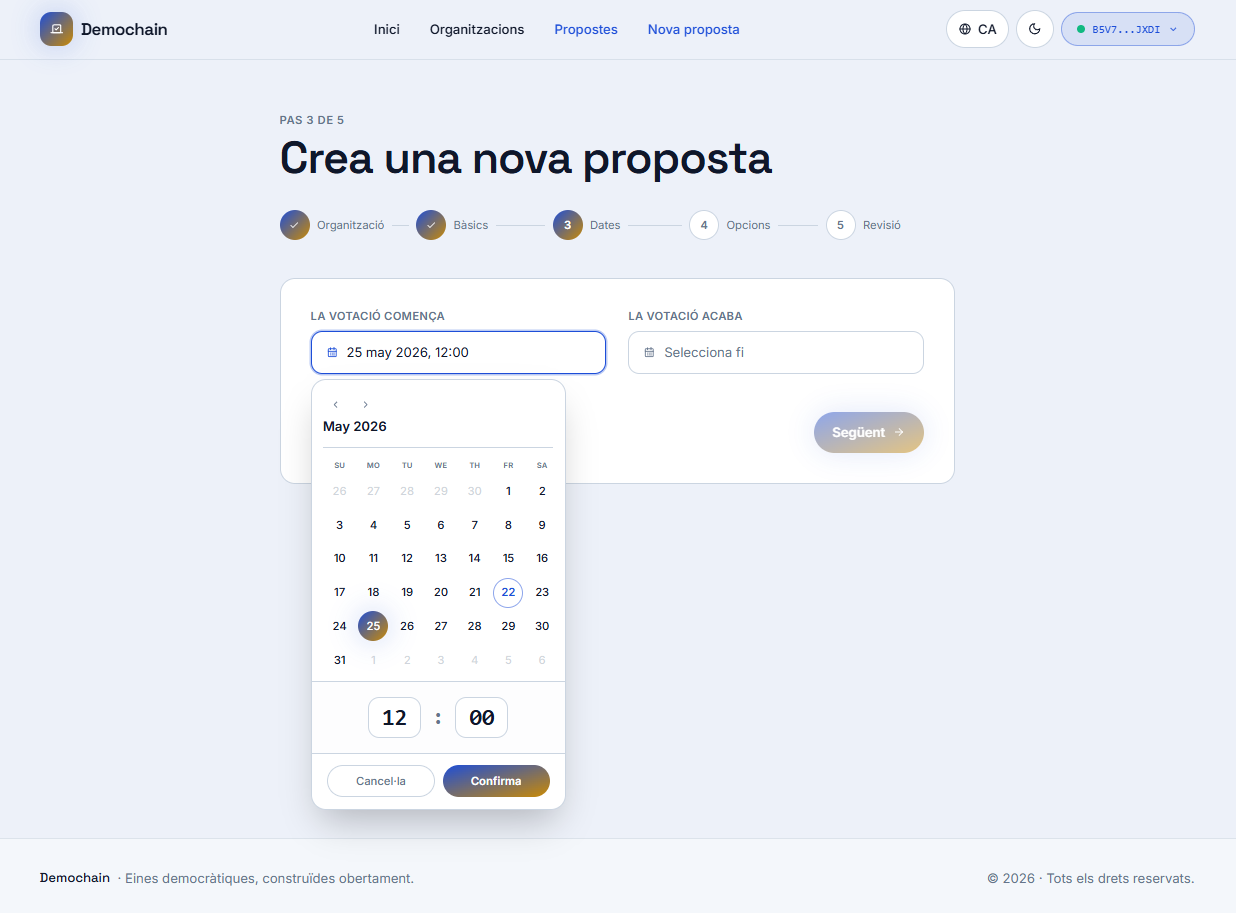
\includegraphics[width=\textwidth]{chapters/images/disseny/screenshots/05-new-proposal-3}
    \caption{Assistent de creació d'una proposta, pas \textit{Dates}.}
    \label{fig:ui-new-proposal-3}
\end{figure}

\begin{figure}[ht]
    \centering
    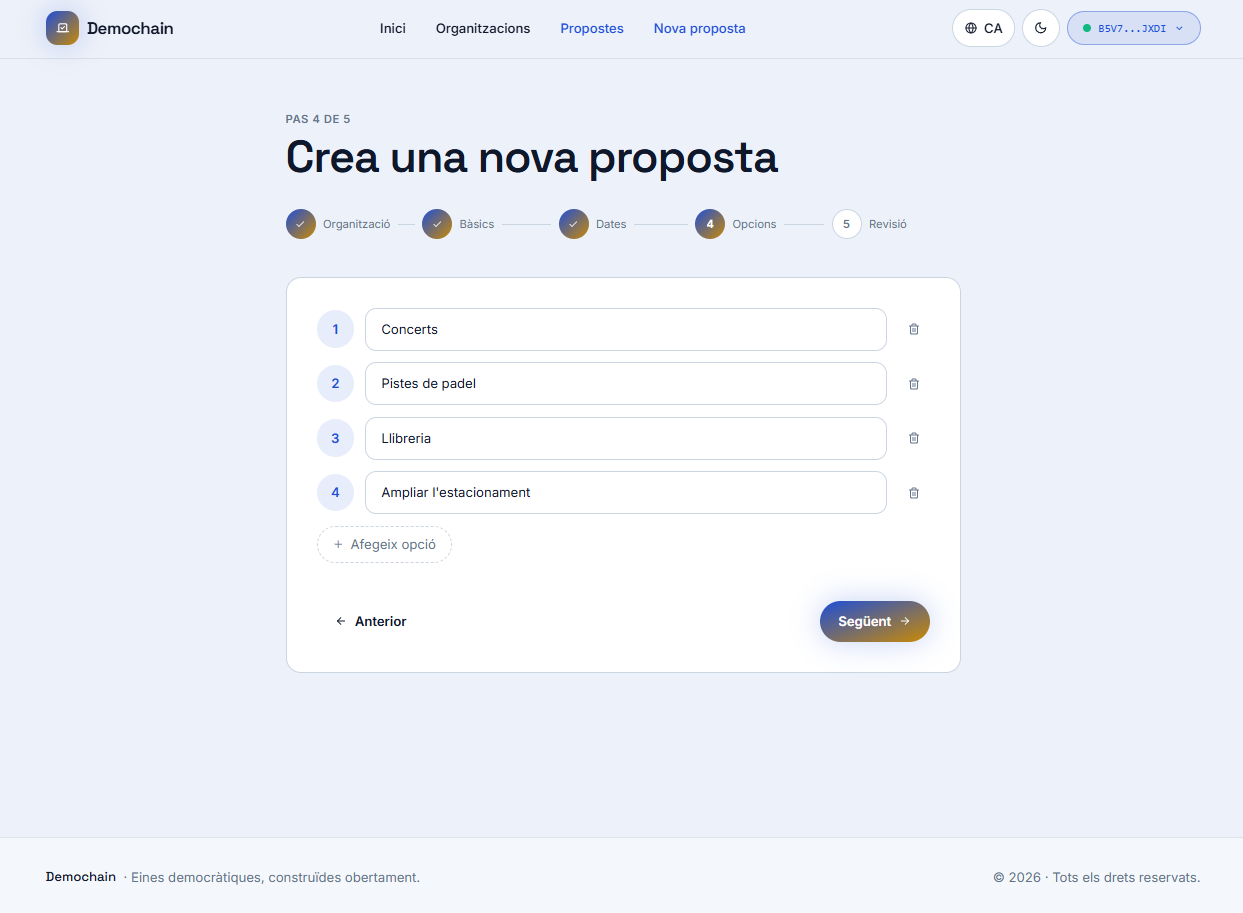
\includegraphics[width=\textwidth]{chapters/images/disseny/screenshots/05-new-proposal-4}
    \caption{Assistent de creació d'una proposta, pas \textit{Opcions}.}
    \label{fig:ui-new-proposal-4}
\end{figure}

\begin{figure}[ht]
    \centering
    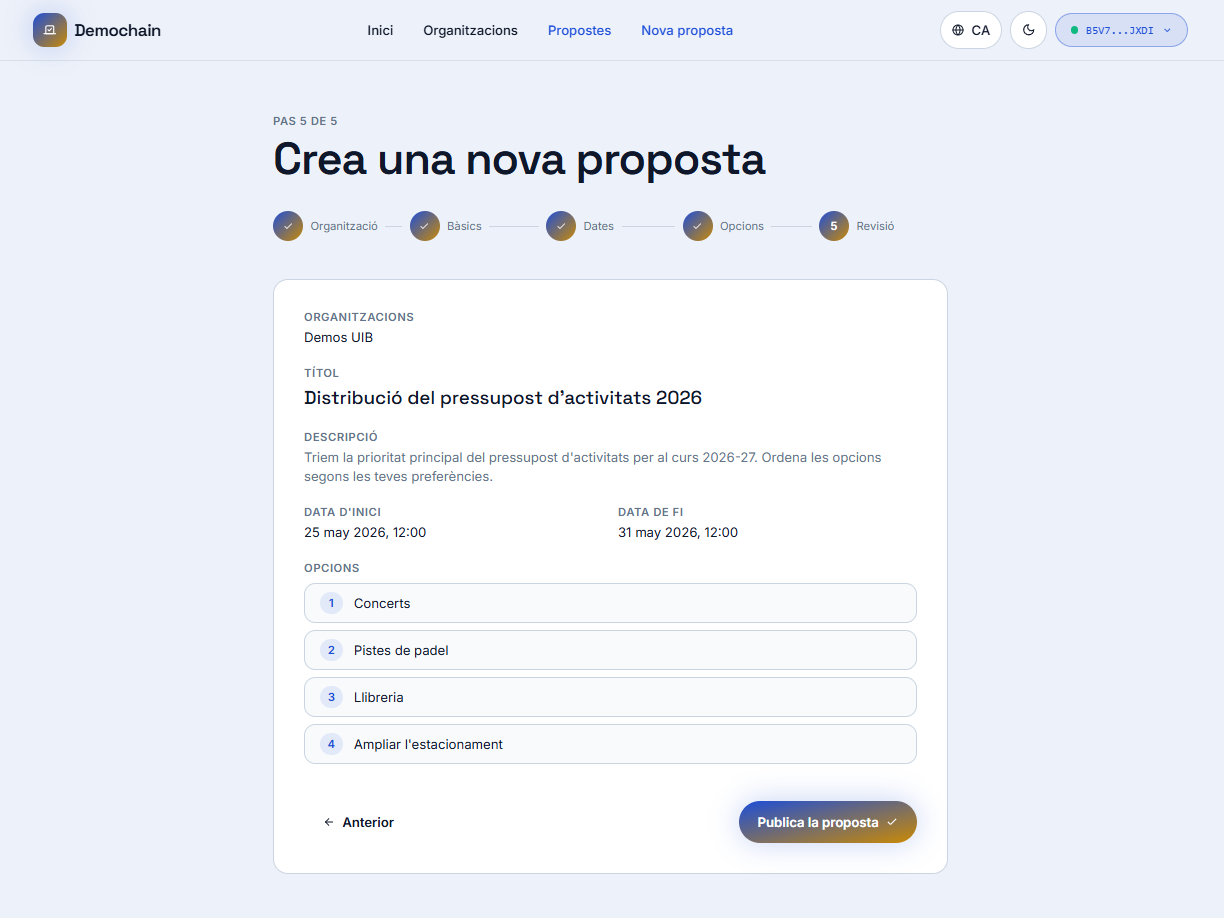
\includegraphics[width=\textwidth]{chapters/images/disseny/screenshots/05-new-proposal-5}
    \caption{Assistent de creació d'una proposta, pas \textit{Revisió}.}
    \label{fig:ui-new-proposal-5}
\end{figure}

\begin{figure}[ht]
    \centering
    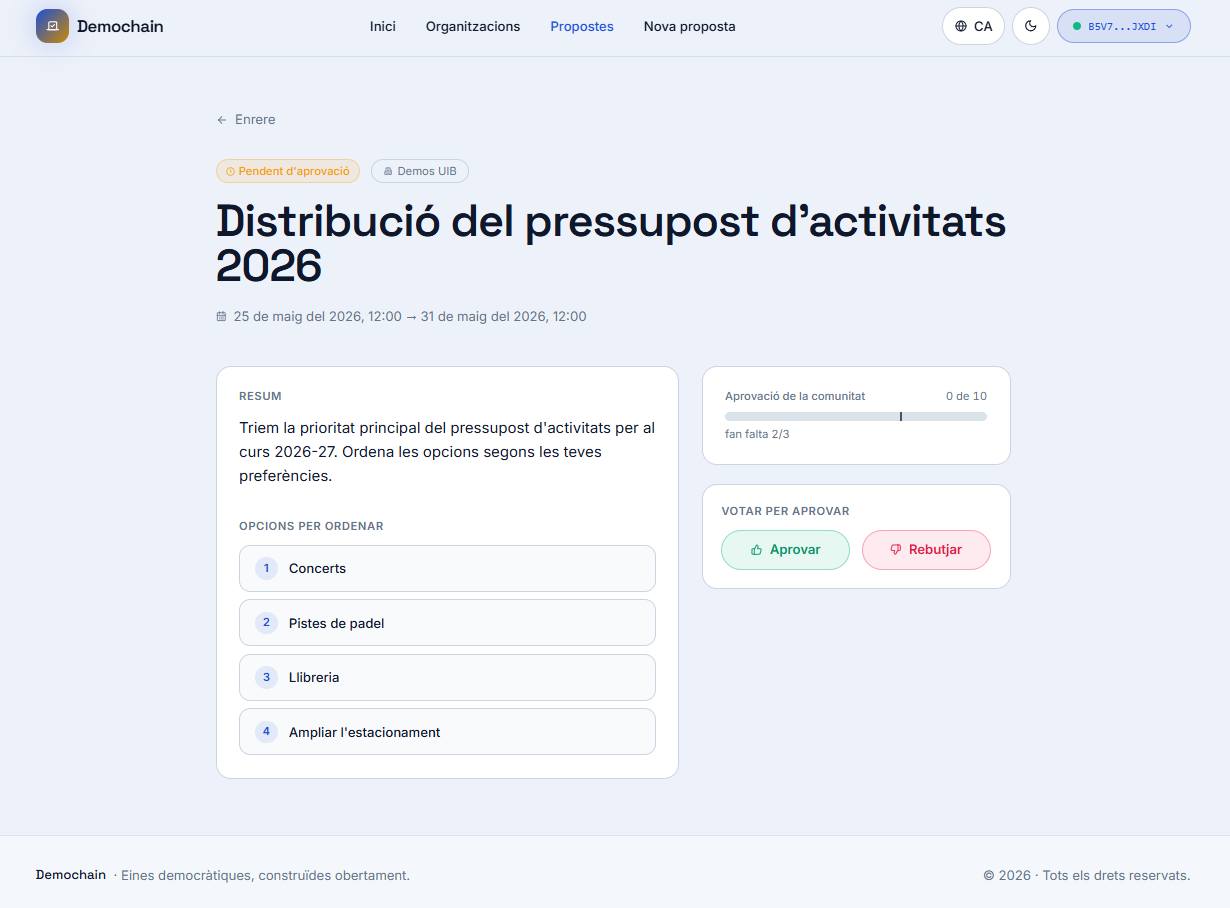
\includegraphics[width=\textwidth]{chapters/images/disseny/screenshots/04b-proposal}
    \caption{Informació concreta d'una proposta: títol, resum, opcions, recompte de vots i formulari per aprobar o rebutjar la proposta.}
    \label{fig:ui-proposal}
\end{figure}

\begin{figure}[ht]
    \centering
    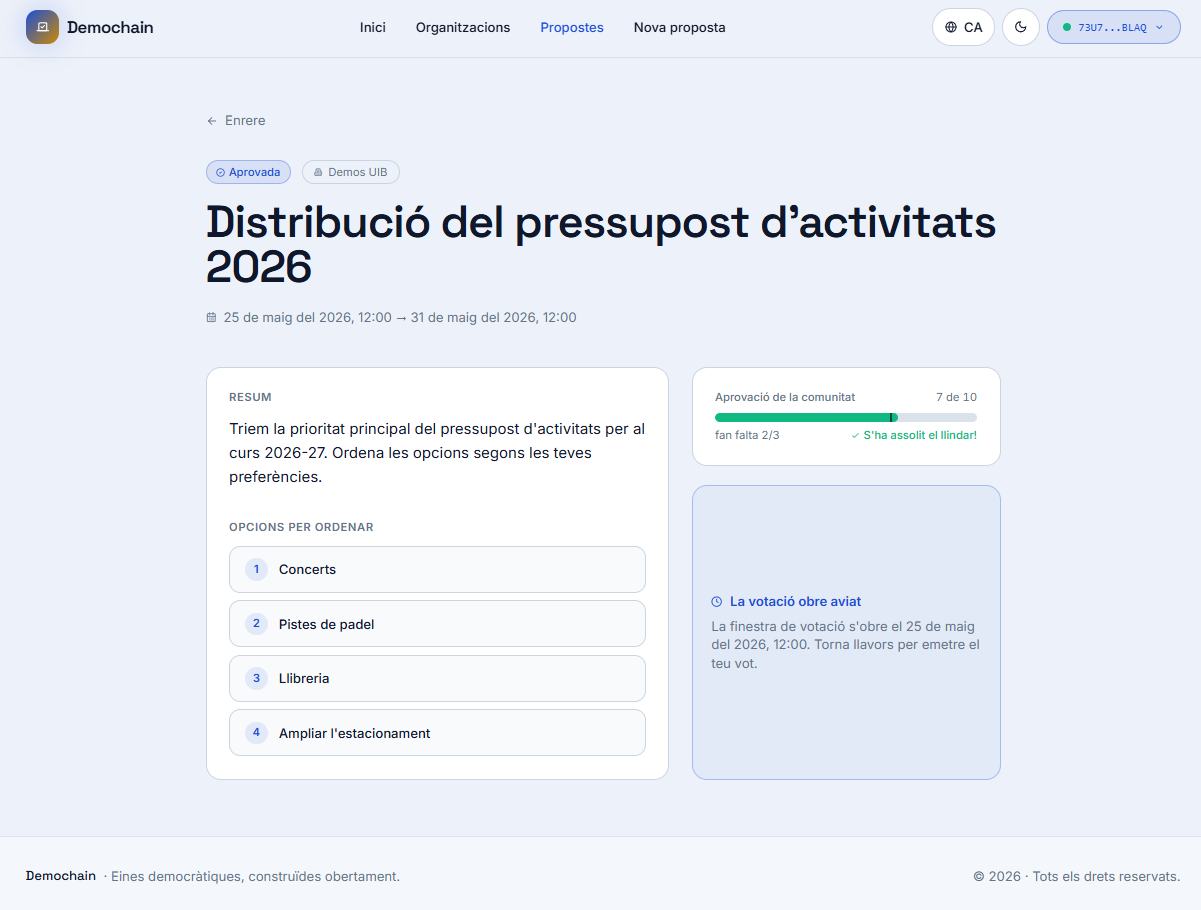
\includegraphics[width=\textwidth]{chapters/images/disseny/screenshots/04c-proposal}
    \caption{Informació concreta d'una proposta que s'ha aprovat i encara no ha començat el període de votació.}
    \label{fig:ui-proposal-aproved}
\end{figure}

\subsection{Emissió de vot}
\label{subsec:emissio-de-vot}

Quan una proposta és aprovada, els membres del cens poden ordenar les opcions arrossegant-les fins a compondre el seu
ranking de preferències.
El component es construeix amb \texttt{@dnd-kit} i admet tant ratolí com teclat, garantint accessibilitat
(\autoref{fig:ui-vote}).
El vot d'elecció es pot modificar tantes vegades com calgui mentre la finestra estigui oberta; en canvi, el vot
d'aprovació previ (binari, visible a la \autoref{fig:ui-proposal}) és immutable un cop emès.
Una vegada emès dona feedback com es veu en la \autoref{fig:ui-vote-confirm} i després passa a una pàgina on pot veure
el seguiment de quanta gent ha votat (\autoref{fig:ui-vote-num}).

\begin{figure}[ht]
    \centering
    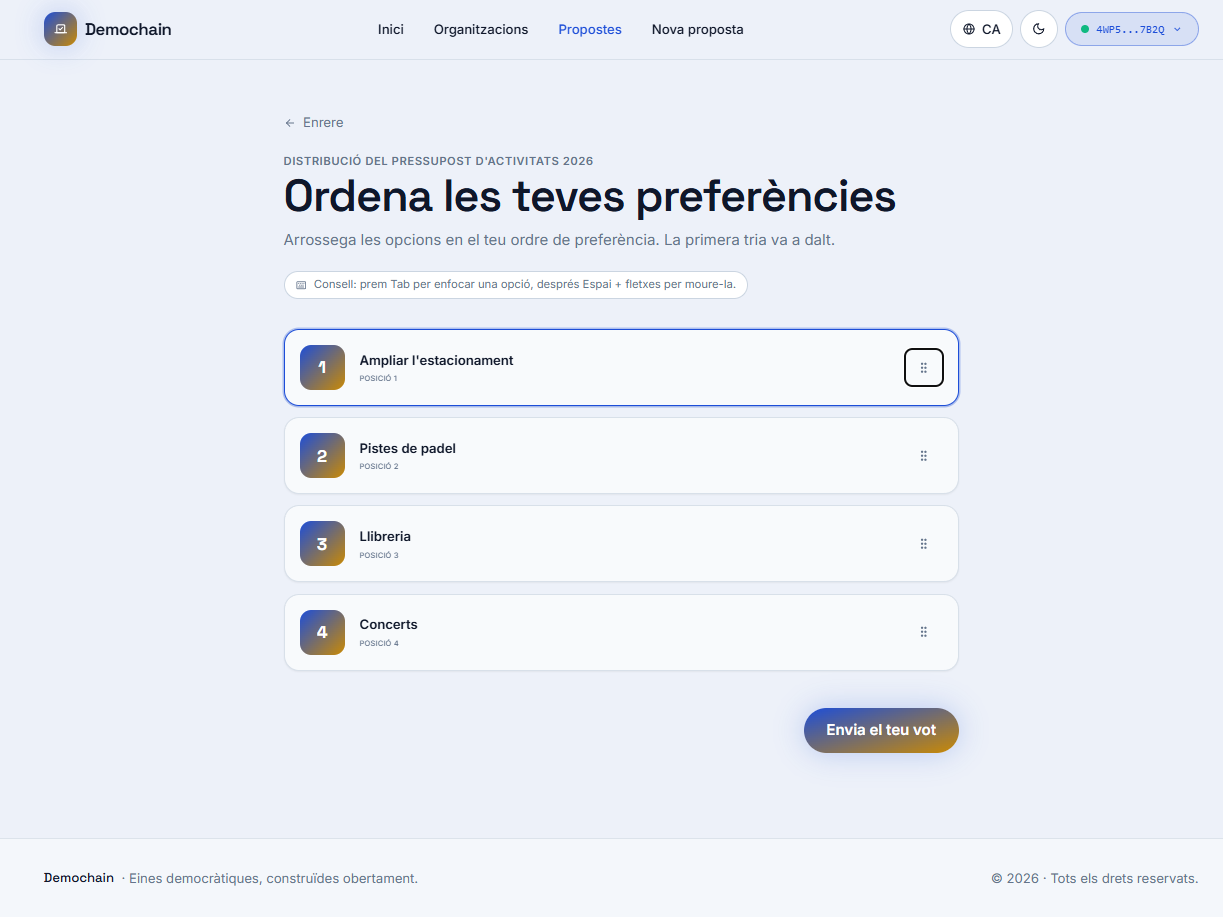
\includegraphics[width=\textwidth]{chapters/images/disseny/screenshots/06-vote-ranking}
    \caption{Pantalla d'emissió de vot: ranking de preferències arrossegables.}
    \label{fig:ui-vote}
\end{figure}

\begin{figure}[ht]
    \centering
    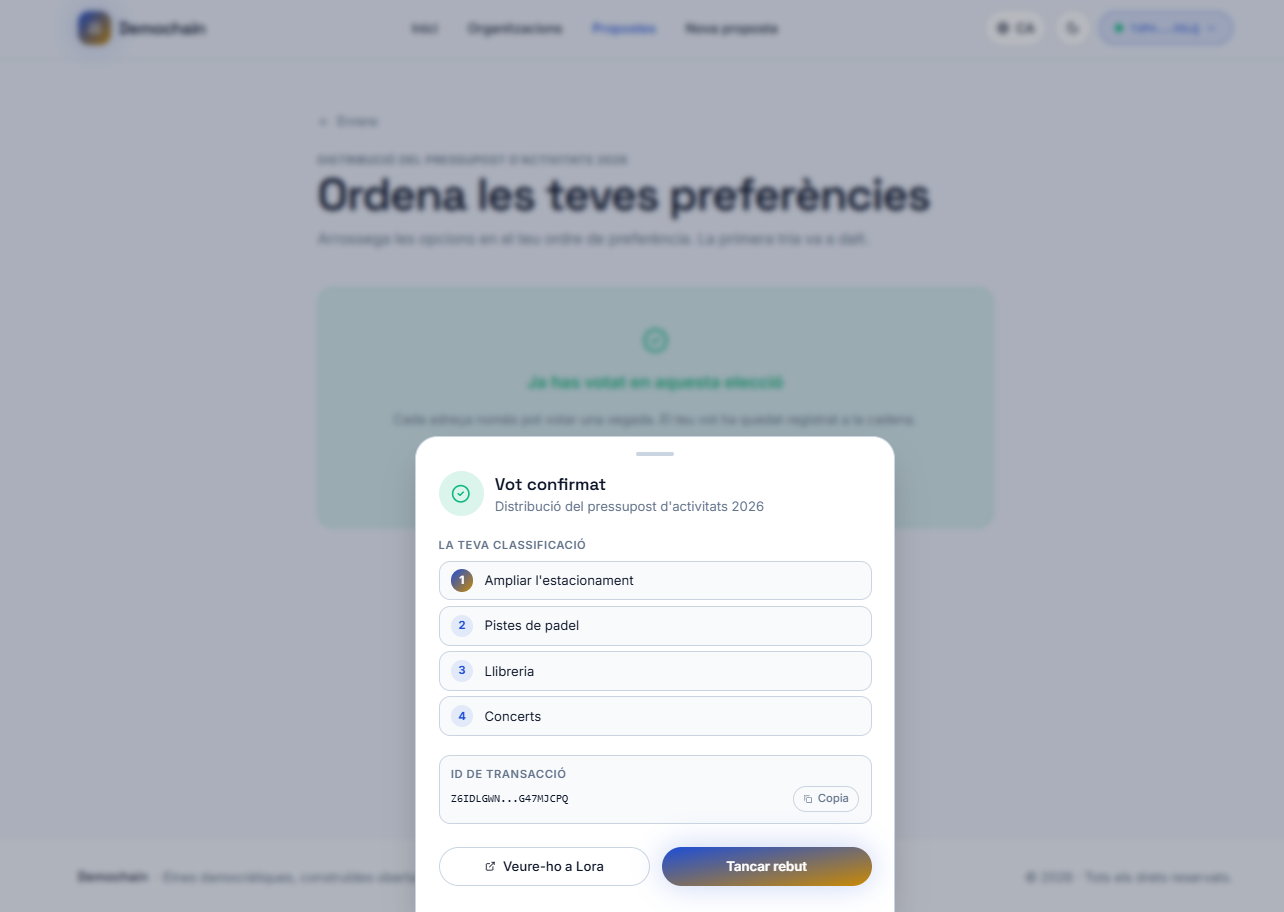
\includegraphics[width=\textwidth]{chapters/images/disseny/screenshots/06b-vote-ranking}
    \caption{Pantalla dde vot confirmat.}
    \label{fig:ui-vote-confirm}
\end{figure}

\begin{figure}[ht]
    \centering
    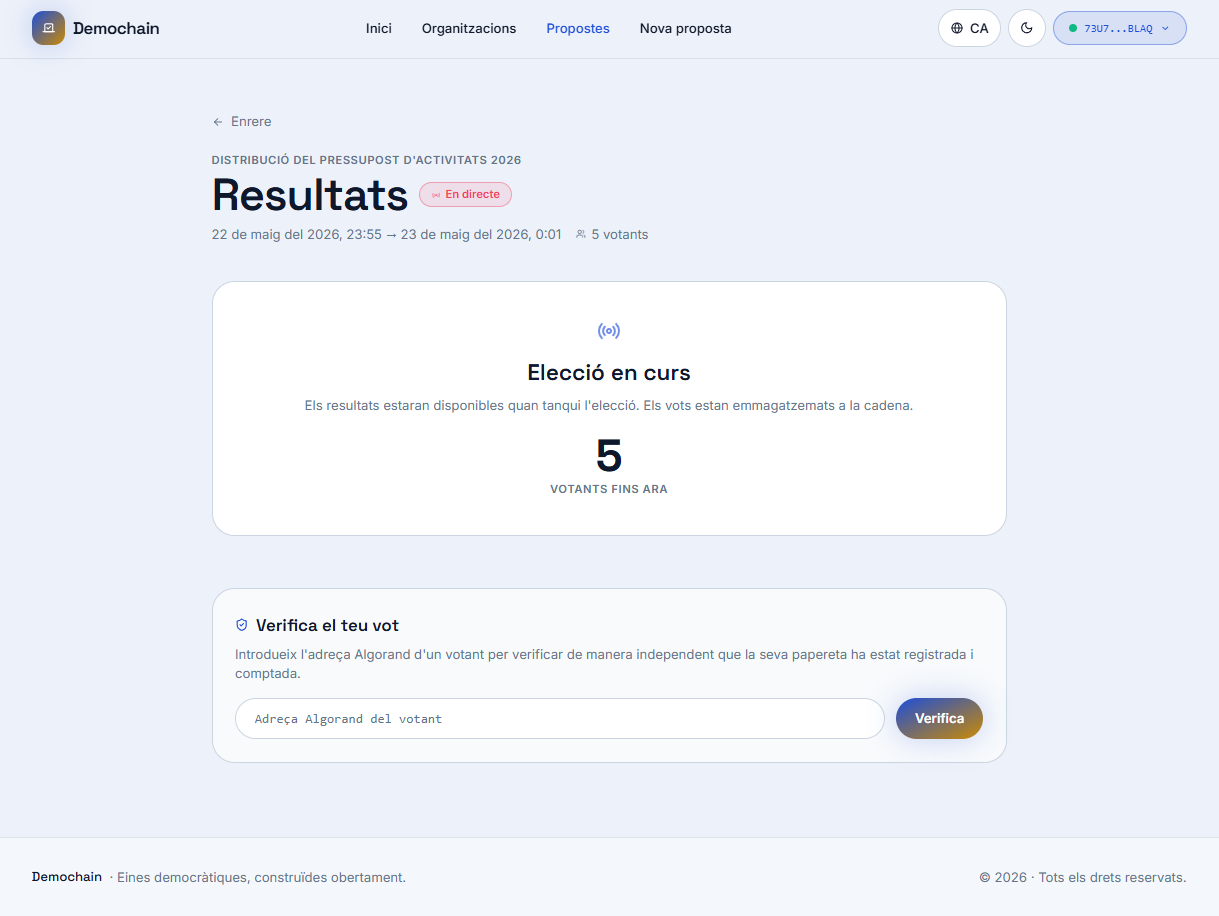
\includegraphics[width=\textwidth]{chapters/images/disseny/screenshots/06c-vote-ranking}
    \caption{Pantalla de seguiment d'enviament de vots}
    \label{fig:ui-vote-num}
\end{figure}

\subsection{Resultats i verificació pública}
\label{subsec:resultats-i-verificacio-publica}

Un cop tancada l'elecció, la pantalla de resultats mostra el ranking final calculat amb el mètode de Schulze
(\autoref{fig:ui-results-1}), així com la matriu de comparacions parelles que permet entendre per què una opció n'ha
vençut una altra (\autoref{fig:ui-results-2}).
El càlcul es fa íntegrament al client a partir de les paperetes llegides de la cadena: el contracte d'Algorand no en
guarda cap resultat precalculat.

\begin{figure}[ht]
    \centering
    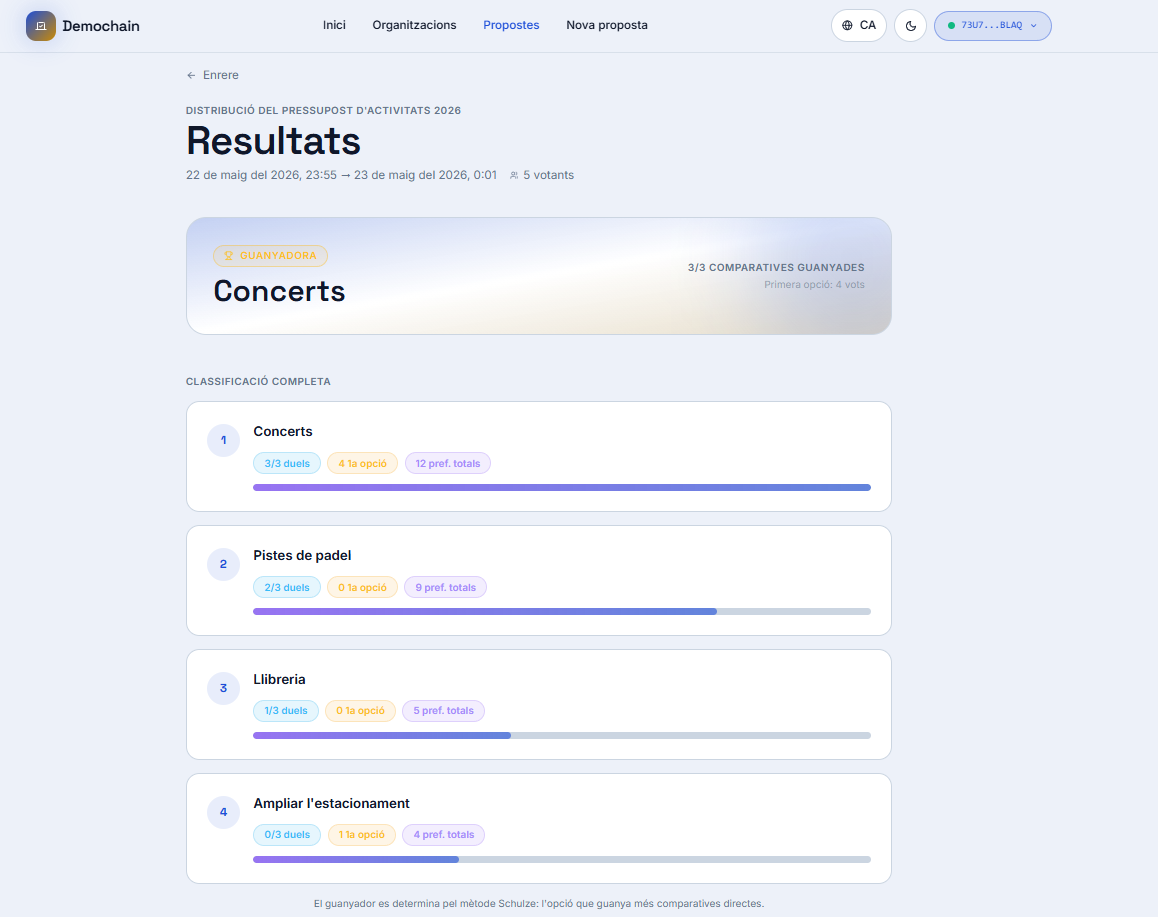
\includegraphics[width=\textwidth]{chapters/images/disseny/screenshots/07-results}
    \caption{Pantalla de resultats finals i verificació pública.}
    \label{fig:ui-results-1}
\end{figure}

\begin{figure}[ht]
    \centering
    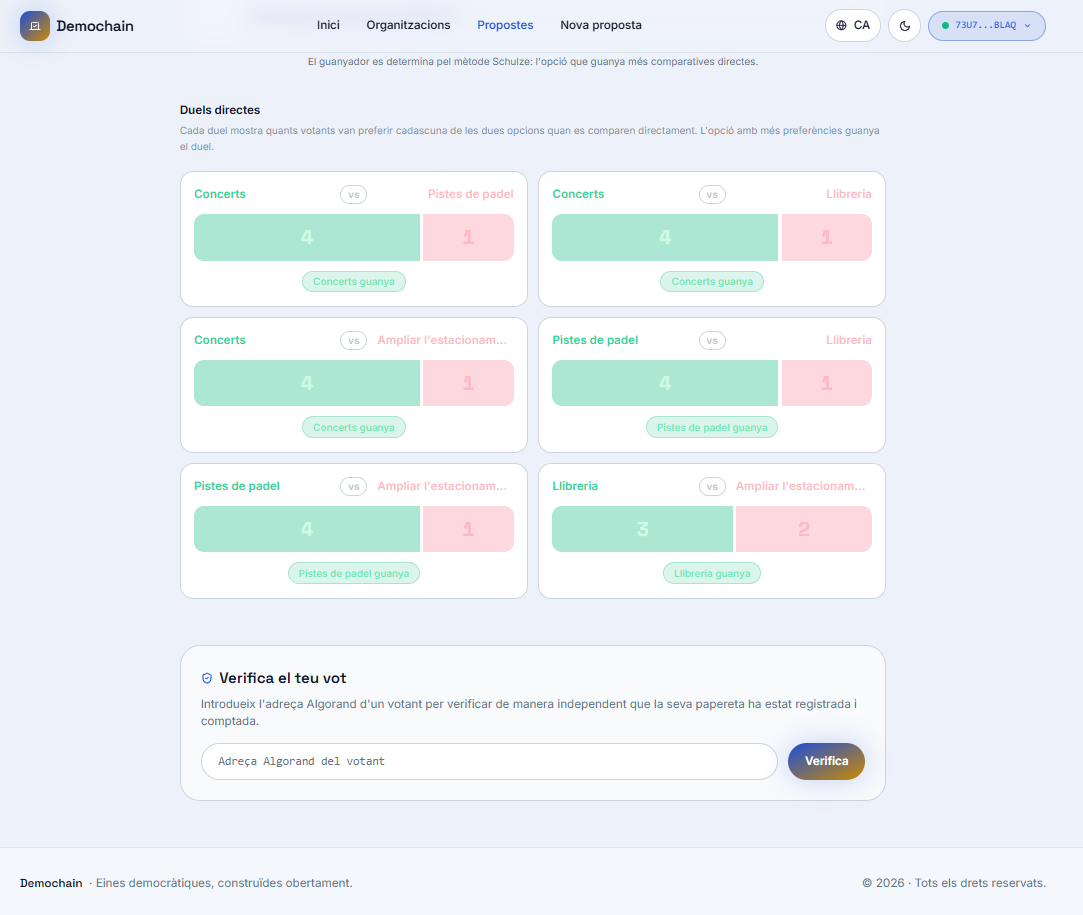
\includegraphics[width=\textwidth]{chapters/images/disseny/screenshots/07b-results}
    \caption{Pantalla de resultats amb els duels directes.}
    \label{fig:ui-results-2}
\end{figure}

A la mateixa pantalla s'hi inclou un panell de verificació obert a qualsevol persona, fins i tot a qui no és membre del
cens.
Introduint una direcció de cartera, el client consulta la blockchain i mostra el ranking que aquella direcció va emetre
o bé indica que no va votar (\autoref{fig:ui-results-3}).
Aquesta funcionalitat, combinada amb l'ancoratge a Ethereum, permet auditar el resultat de manera independent.

\begin{figure}[ht]
    \centering
    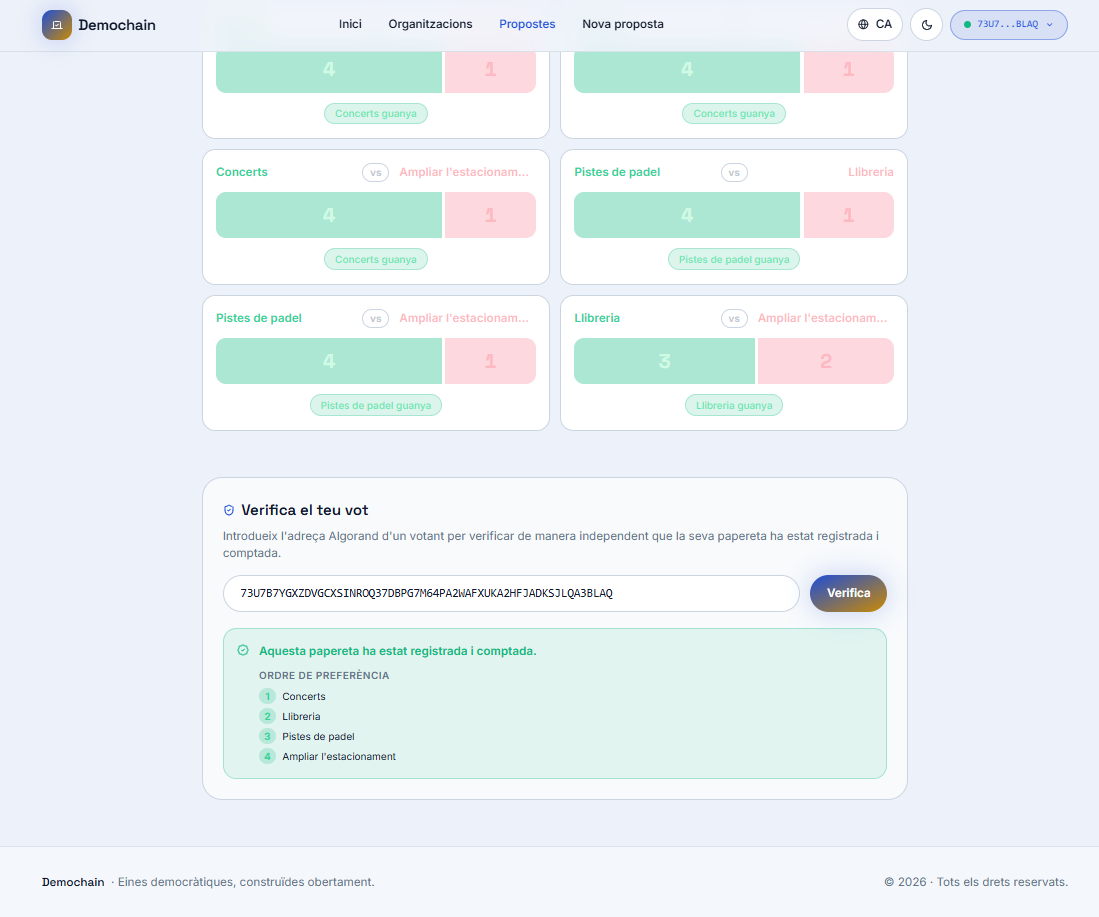
\includegraphics[width=\textwidth]{chapters/images/disseny/screenshots/07c-results}
    \caption{Pantalla de verificació del vot que s'ha emès una vegada acabada l'elecció.}
    \label{fig:ui-results-3}
\end{figure}


\section{Flux de comunicació amb l'usuari}
\label{sec:flux-de-comunicacio-amb-l'usuari}

Aquesta secció recull els fluxos de comunicació més rellevants entre l'administrador, el votant, el client, la cartera i
la cadena.
Estan representats com a diagrames de seqüència UML i s'han generat a partir de les especificacions Mermaid incloses al
repositori.

\subsection{Gestió d'organitzacions}
\label{subsec:gestio-d'organitzacions}

Aquest flux agrupa les tres operacions que pot fer un administrador sobre una organització: crear-la, donar d'alta noves
adreces al cens i eliminar-ne (\autoref{fig:seq-organization}).
La part més rellevant del disseny és com el client amaga al votant la limitació tècnica del contracte, que només admet
un màxim de set adreces per transacció de cens.
Quan l'administrador carrega un \ac{CSV} amb molts membres, el client el trosseja internament en lots de set i
sol·licita la signatura de tantes transaccions com calgui, mostrant una barra de progrés.
D'aquesta manera, l'única conseqüència visible per a l'administrador és que els censos molt grans tarden una mica més a
confirmar-se.

A més, el contracte aplica dues regles invariants que també queden reflectides al diagrama: només l'administrador pot
modificar el cens i mai pot eliminar-se ell mateix, ja que tota organització ha de tenir com a mínim un membre.

\begin{figure}[ht]
    \centering
    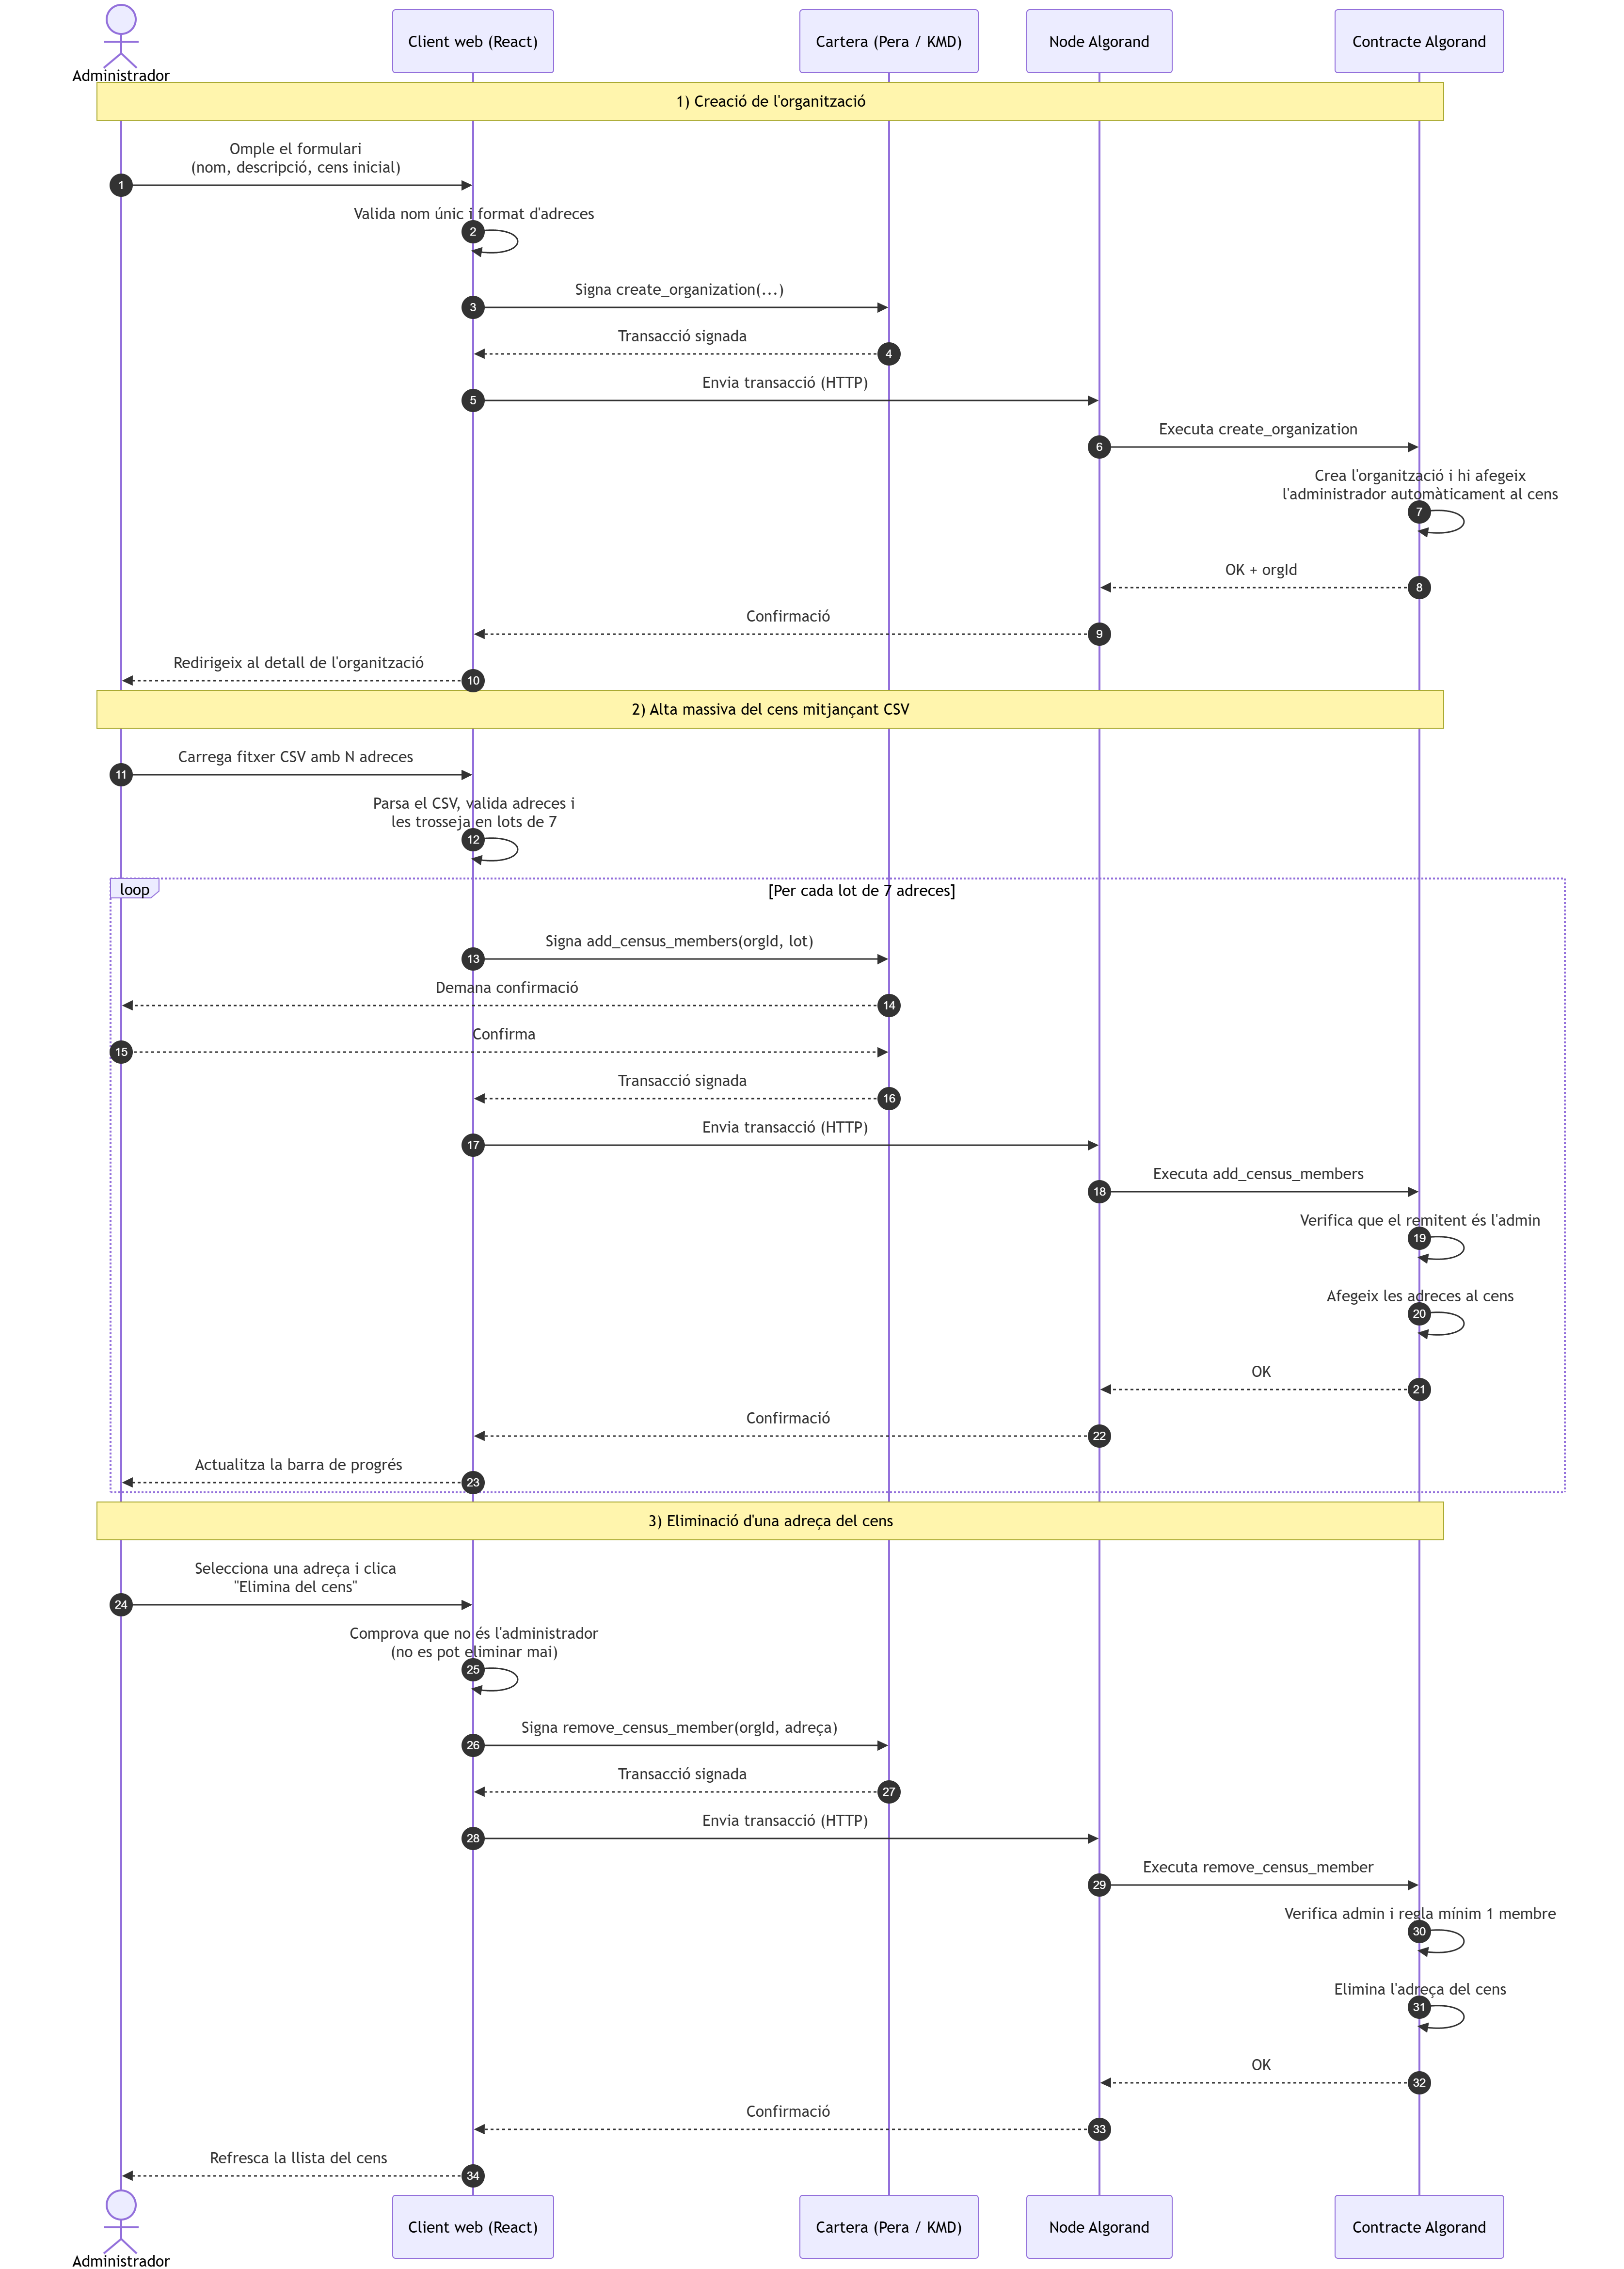
\includegraphics[width=\textwidth]{chapters/images/disseny/sequences/seq-organization}
    \caption{Diagrama de seqüència: creació d'una organització i gestió del seu cens (alta massiva via CSV i baixa individual).}
    \label{fig:seq-organization}
\end{figure}

\subsection{Crear una proposta}
\label{subsec:crear-una-proposta}

El flux comença al formulari guiat del client.
Un cop l'usuari ha completat els cinc passos, el client construeix la transacció \ac{ABI} corresponent i en sol·licita
la signatura a la cartera.
La transacció signada s'envia al node Algorand i, en cas d'èxit, el contracte valida les restriccions (cens, dates,
opcions) i registra la proposta a Box Storage.
El client invalida la seva caché per recollir l'estat actualitzat i mostra la proposta acabada de crear en estat
\textit{PendingApproval}.

\begin{figure}[ht]
    \centering
    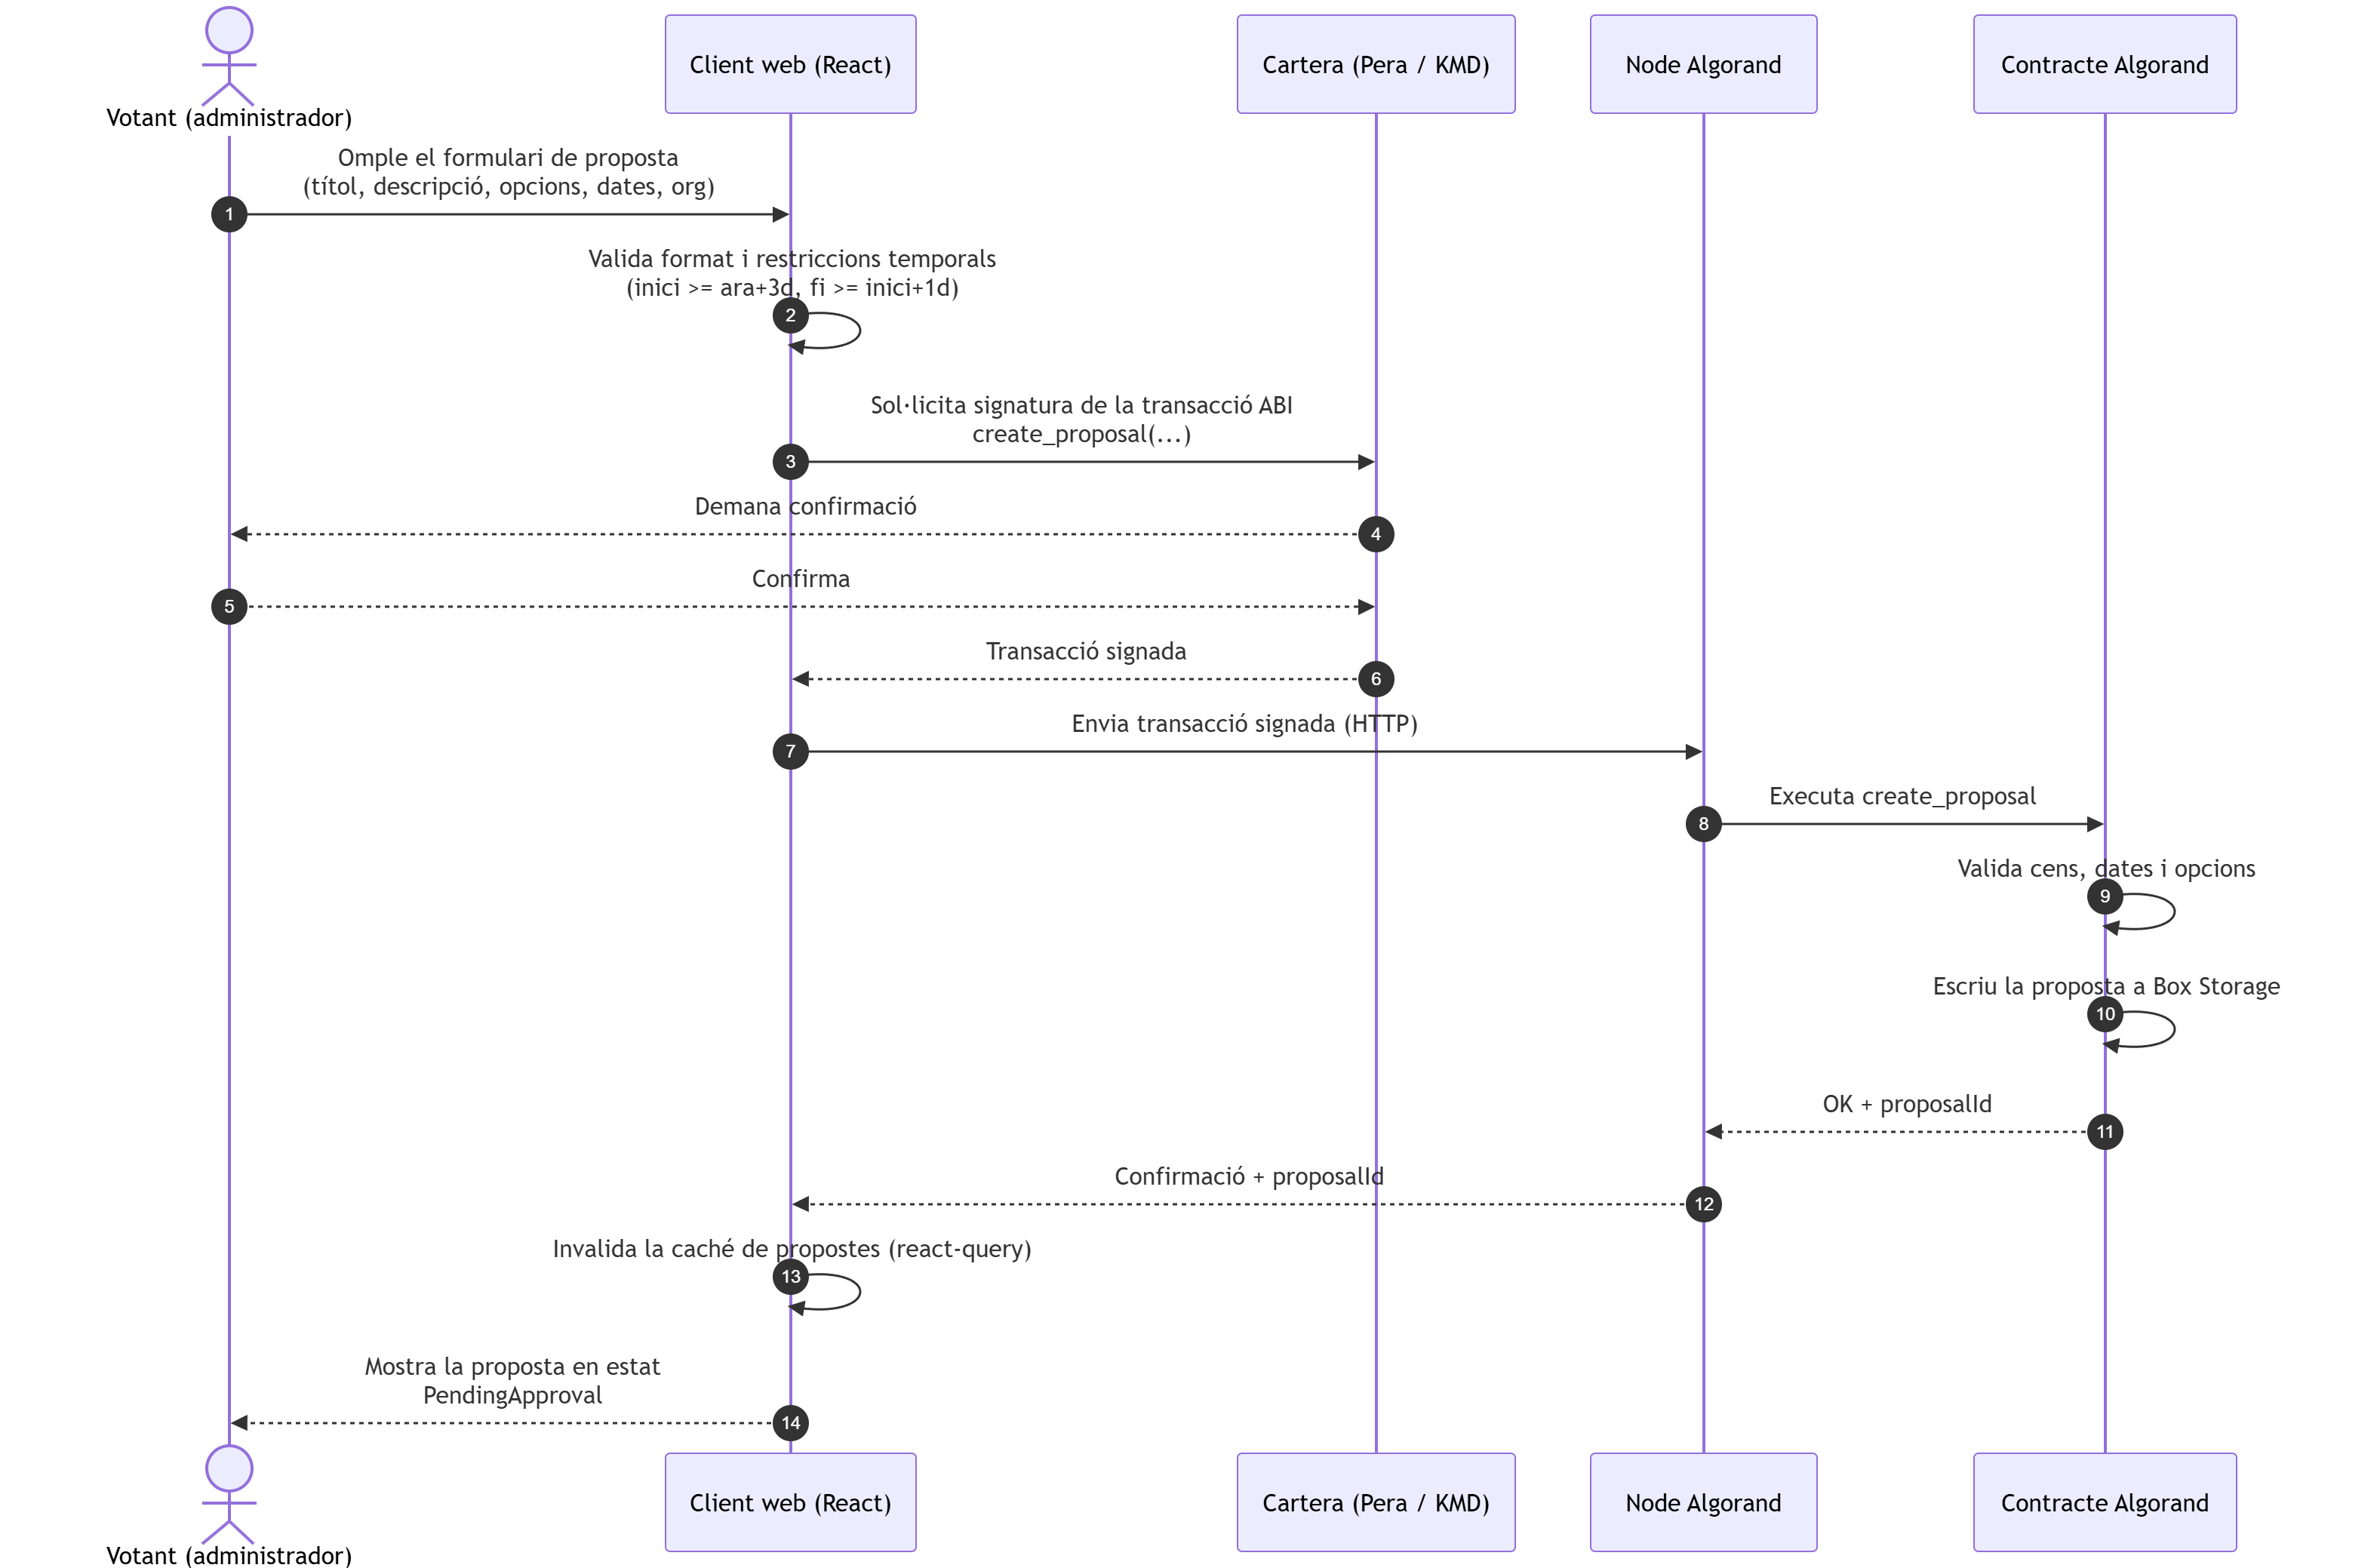
\includegraphics[width=\textwidth]{chapters/images/disseny/sequences/seq-create-proposal}
    \caption{Diagrama de seqüència: creació d'una proposta.}
    \label{fig:seq-create-proposal}
\end{figure}

\subsection{Votar l'aprovació d'una proposta}
\label{subsec:votar-l'aprovacio-d'una-proposta}

El vot d'aprovació és binari (a favor o en contra) i immutable.
El client comprova que la proposta es troba en estat \textit{PendingApproval} i que falten més de tres dies per a la
data d'inici; en cas contrari, no permet emetre el vot.
El contracte verifica que el votant pertany al cens i que no ha votat amb anterioritat.
Aquest disseny és deliberadament conservador: vol garantir que el resultat de la fase d'aprovació es coneix amb prou
antelació perquè ningú es pugui sorprendre que una proposta passi (o no passi) a elecció a última hora.

\begin{figure}[ht]
    \centering
    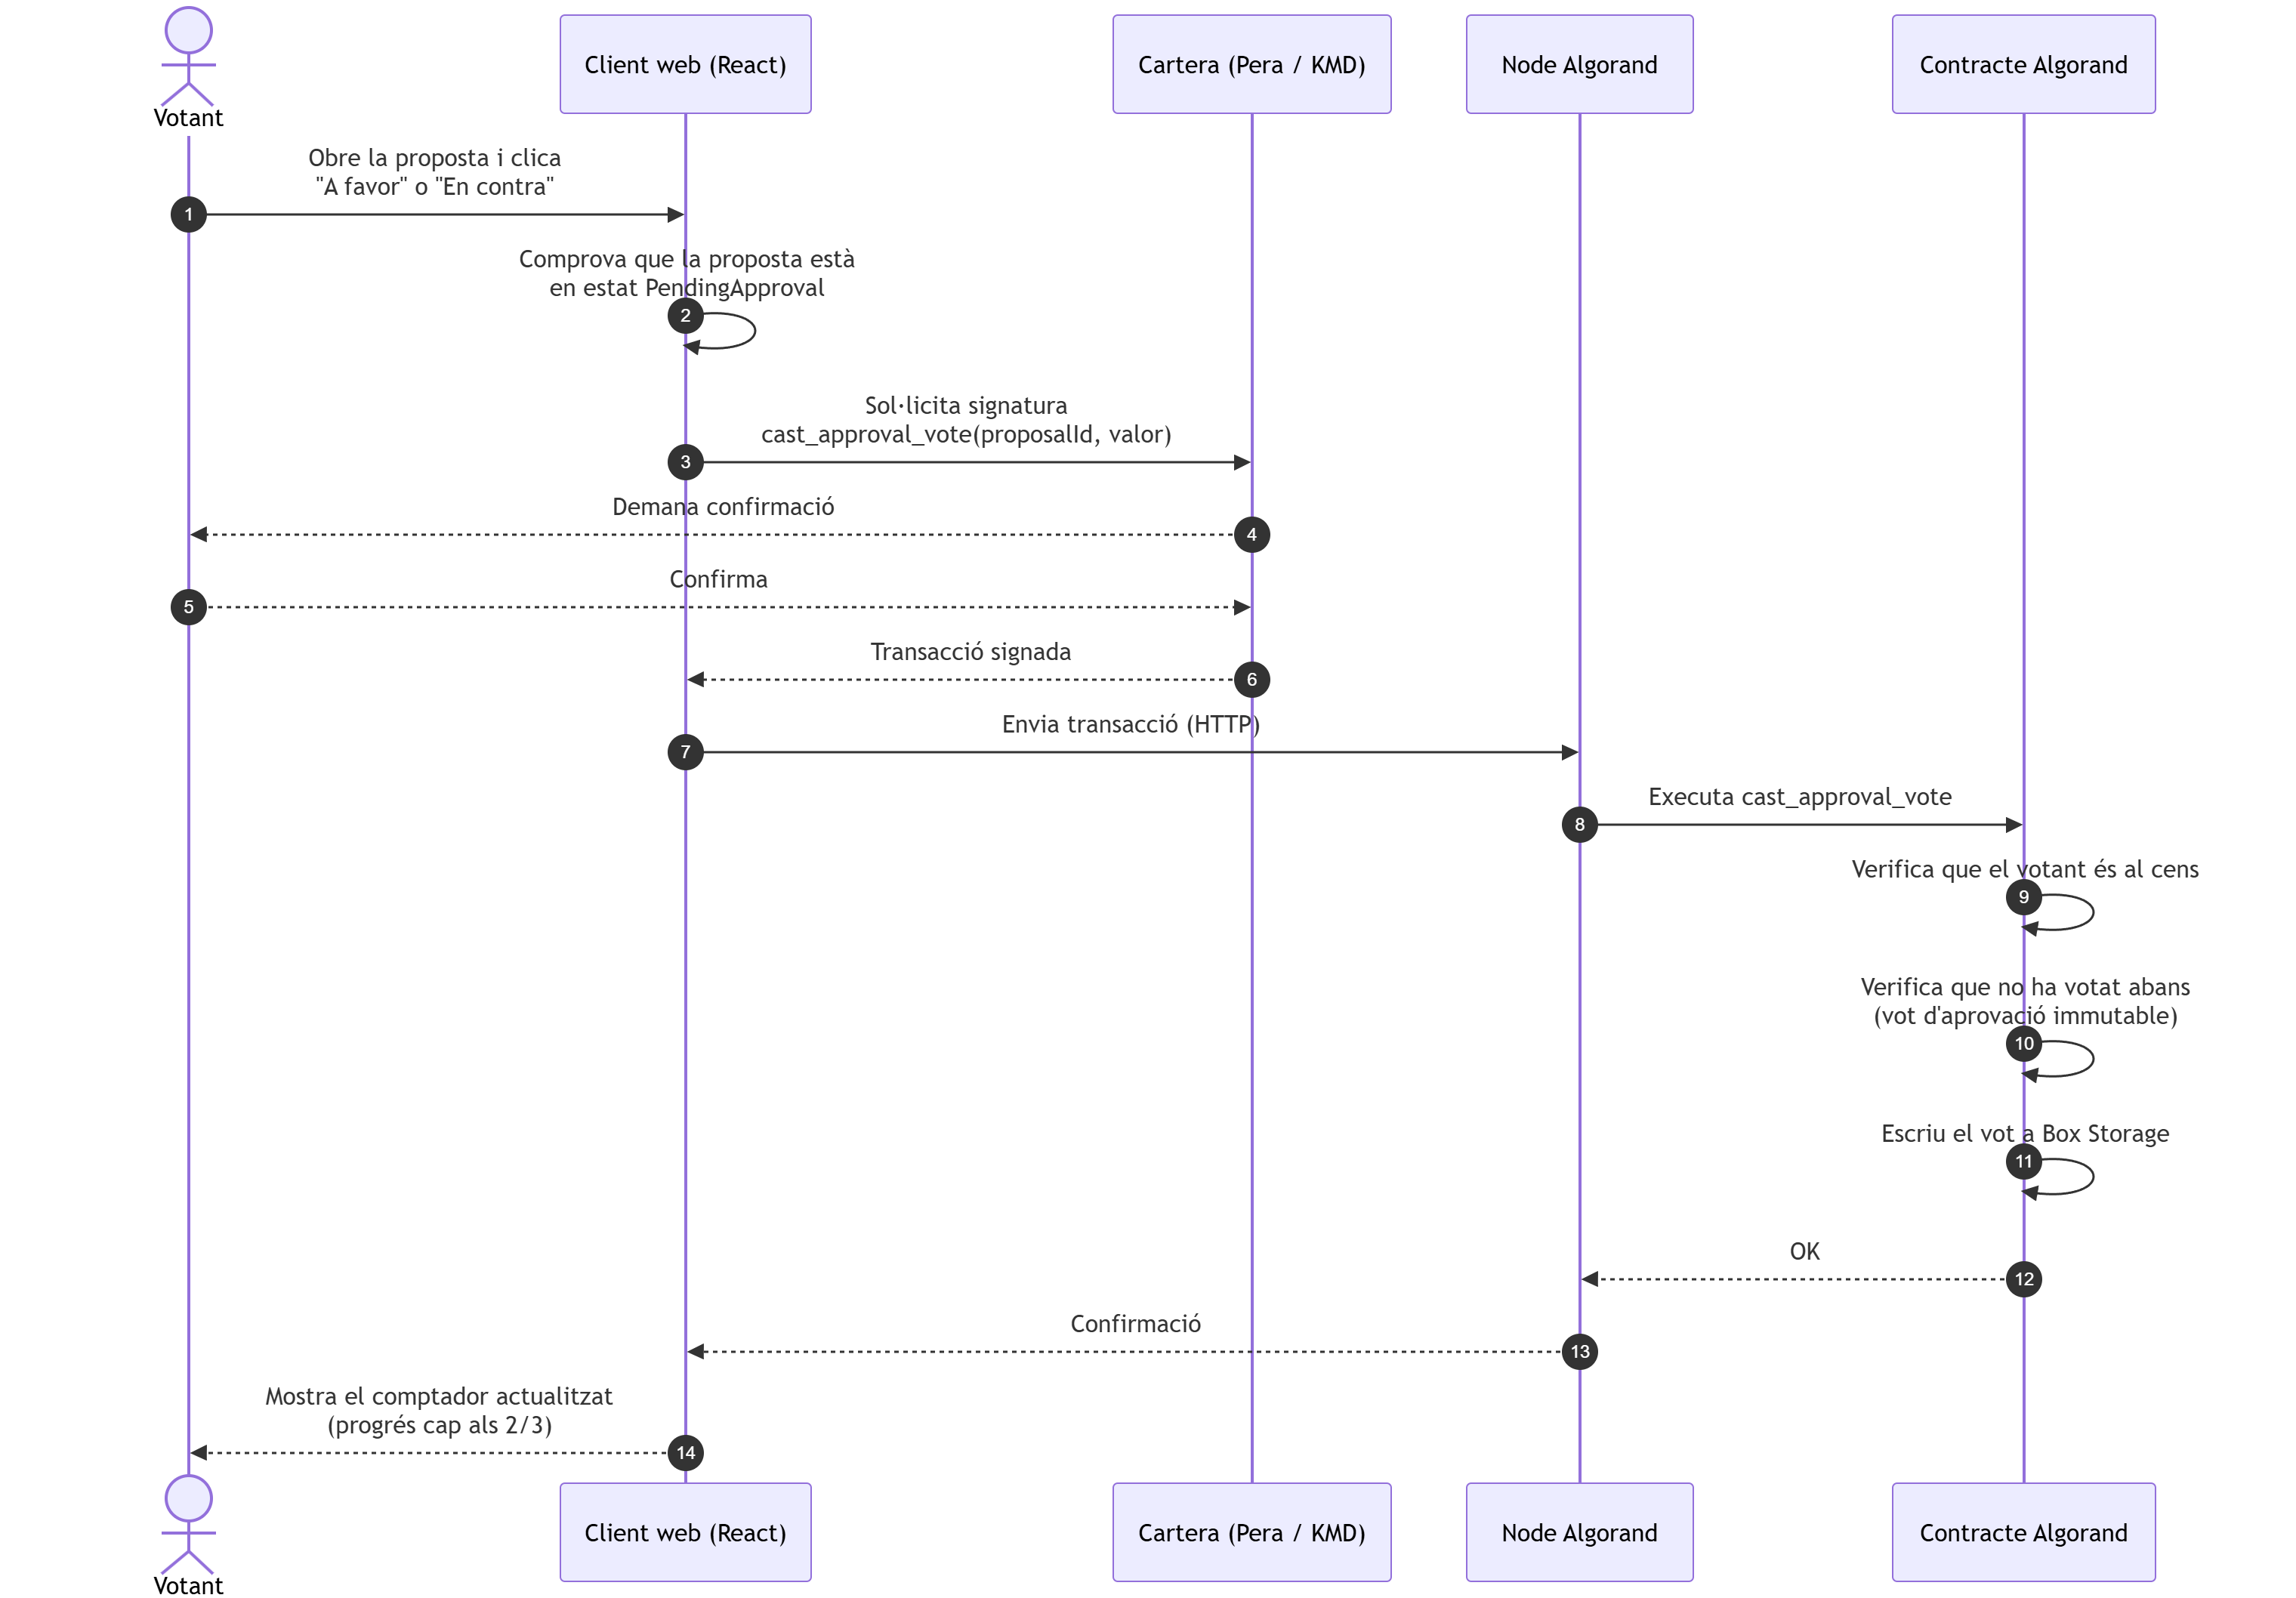
\includegraphics[width=\textwidth]{chapters/images/disseny/sequences/seq-approval-vote}
    \caption{Diagrama de seqüència: vot d'aprovació.}
    \label{fig:seq-approval-vote}
\end{figure}

\subsection{Emetre el vot d'elecció (ranking)}
\label{subsec:emetre-el-vot-d'eleccio-(ranking)}

Quan la proposta entra a l'estat \textit{Open}, el votant pot ordenar les opcions segons les seves preferències.
A diferència del vot d'aprovació, el ranking sí que es pot modificar tantes vegades com calgui mentre l'elecció estigui
oberta.
El contracte sobreescriu el vot anterior amb cada nova transacció, però en deixa traça a la cadena perquè qualsevol
verificació externa només considera l'última versió.

\begin{figure}[ht]
    \centering
    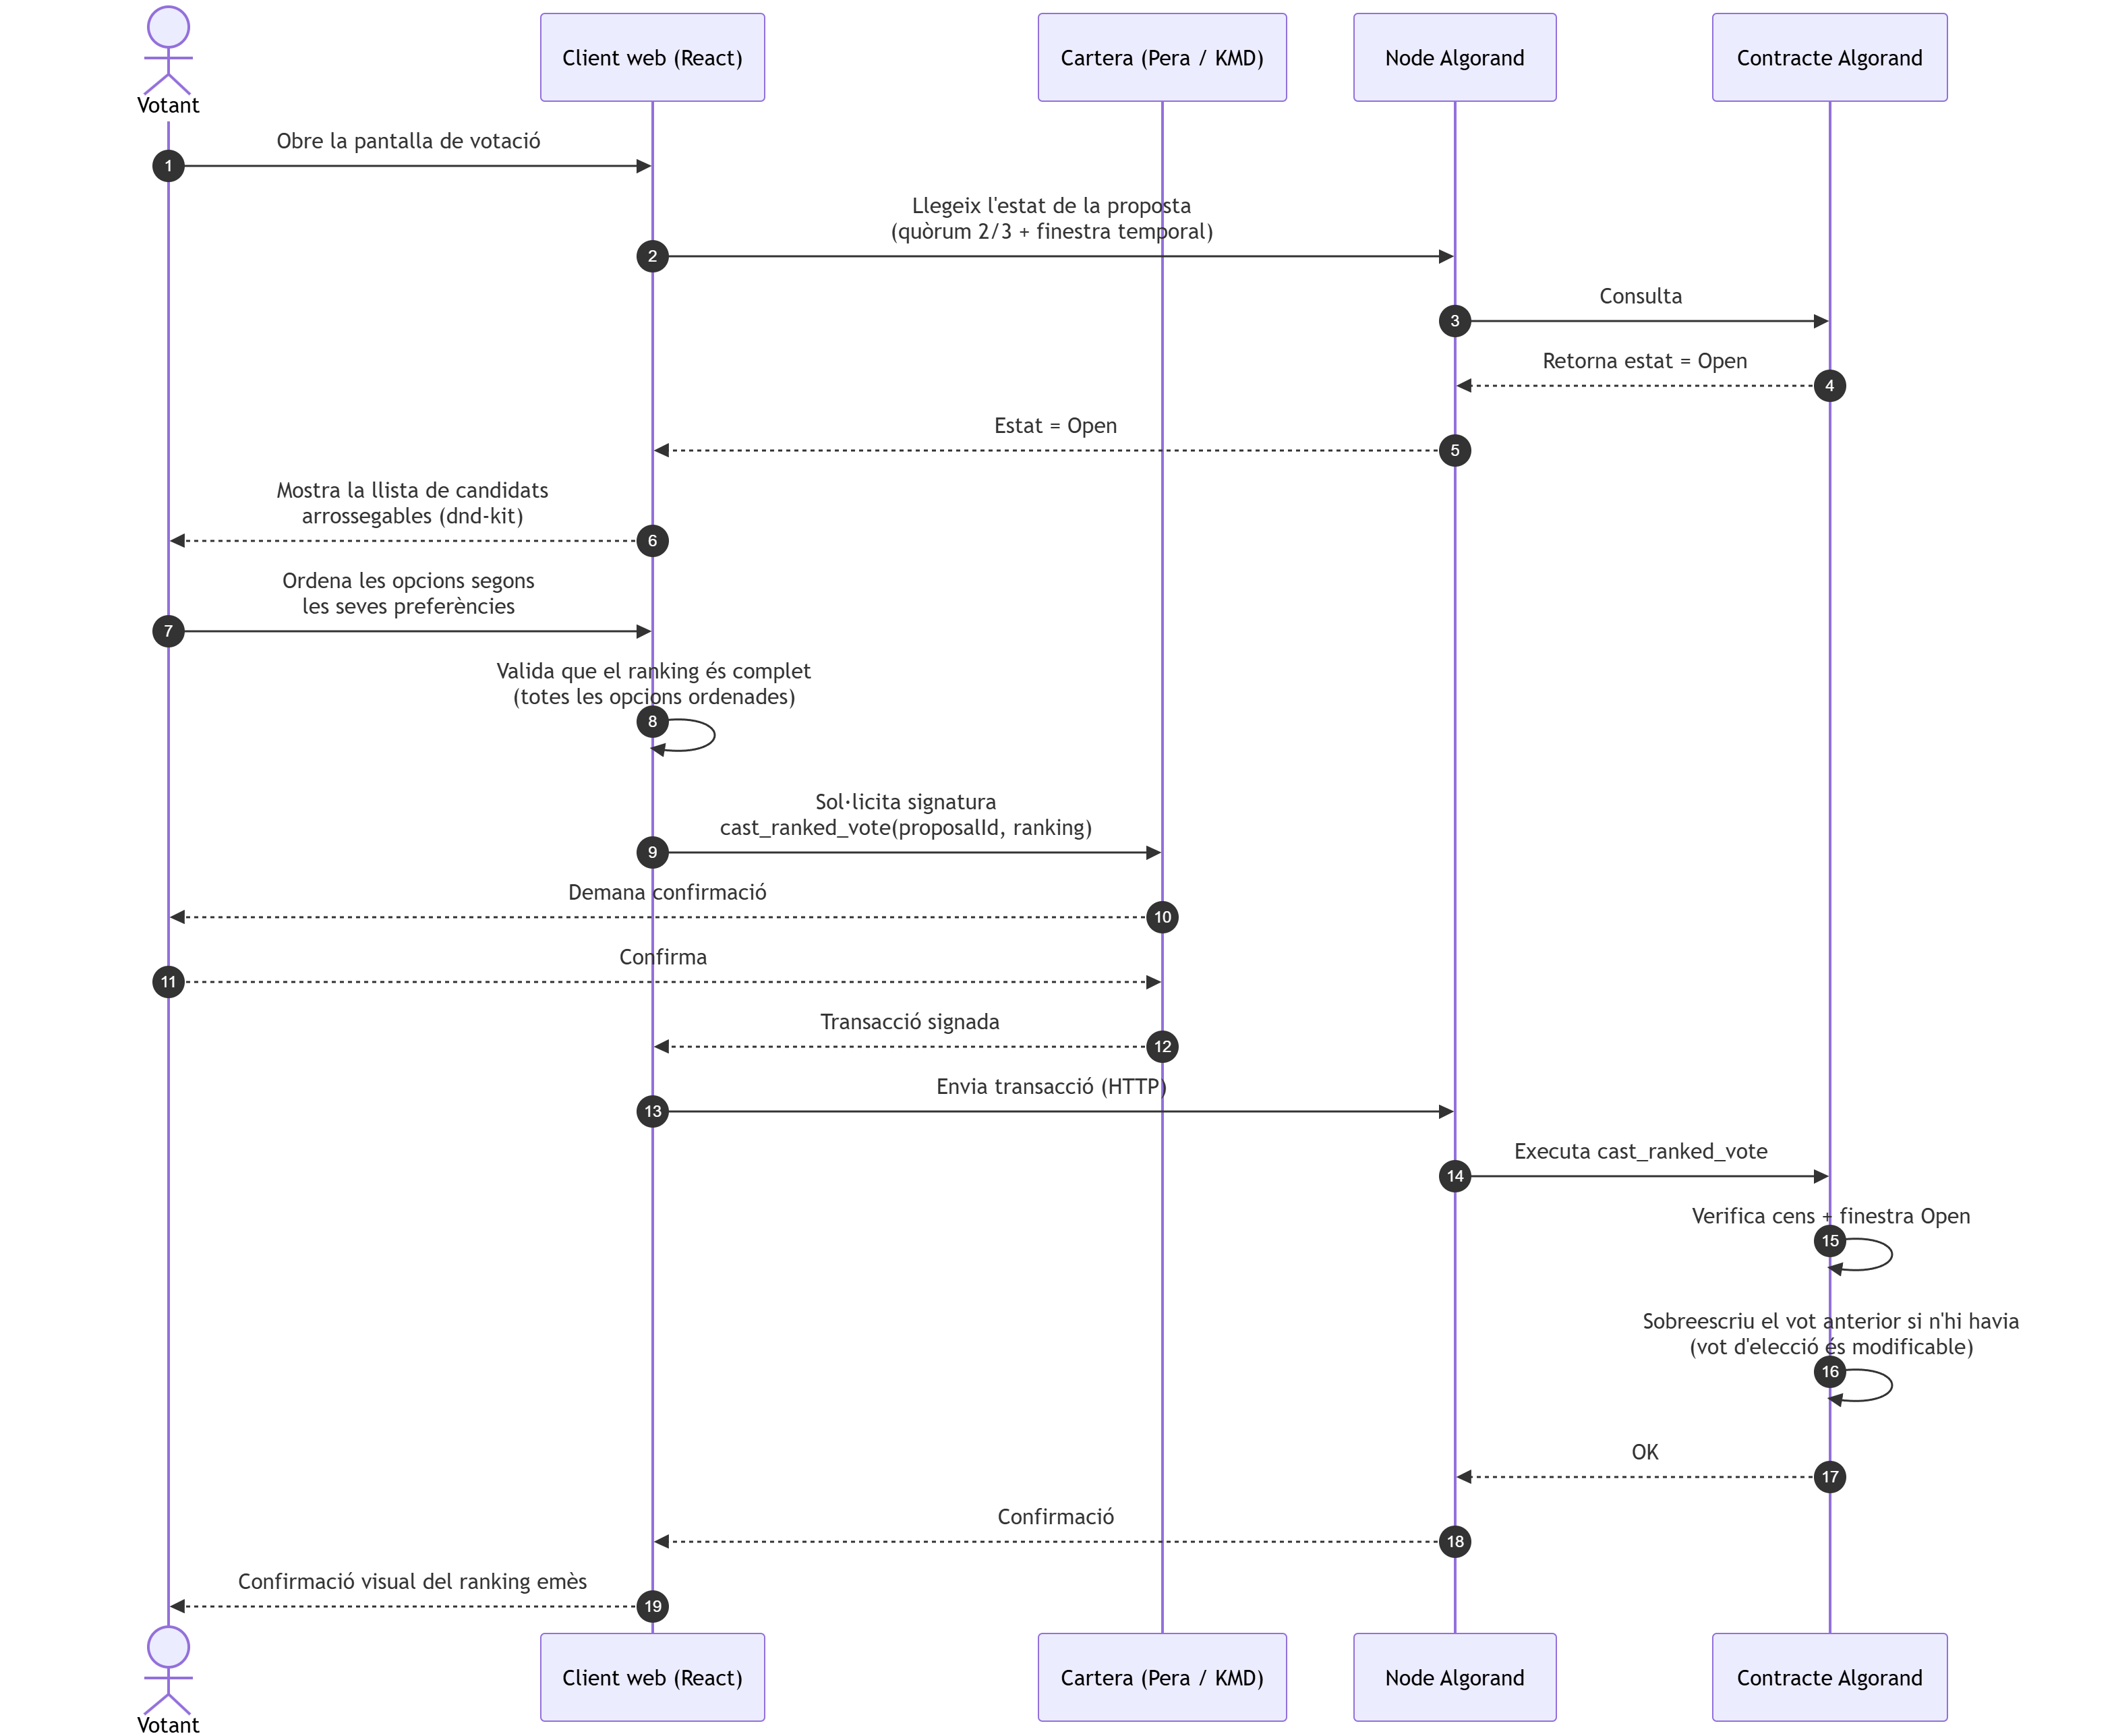
\includegraphics[width=\textwidth]{chapters/images/disseny/sequences/seq-ranked-vote}
    \caption{Diagrama de seqüència: vot d'elecció amb ranking.}
    \label{fig:seq-ranked-vote}
\end{figure}


\section{Flux autònom i automàtic}
\label{sec:flux-autonom-i-automatic}

\subsection{Ancoratge a Ethereum}
\label{subsec:ancoratge-a-ethereum}

Aquest flux s'executa automàticament i paral·lelament a cada node un cop una elecció es tanca.
Tots els nodes llegeixen les paperetes del contracte d'Algorand, en deriven independentment el mateix \textit{hash}
determinista i l'envien al \textit{NotaryContract} d'Ethereum.
El contracte acumula els enviaments fins que K nodes coincideixen en el mateix \textit{hash}; en aquell moment registra
l'elecció com a ancorada de manera permanent i emet un esdeveniment públic.

\begin{figure}[ht]
    \centering
    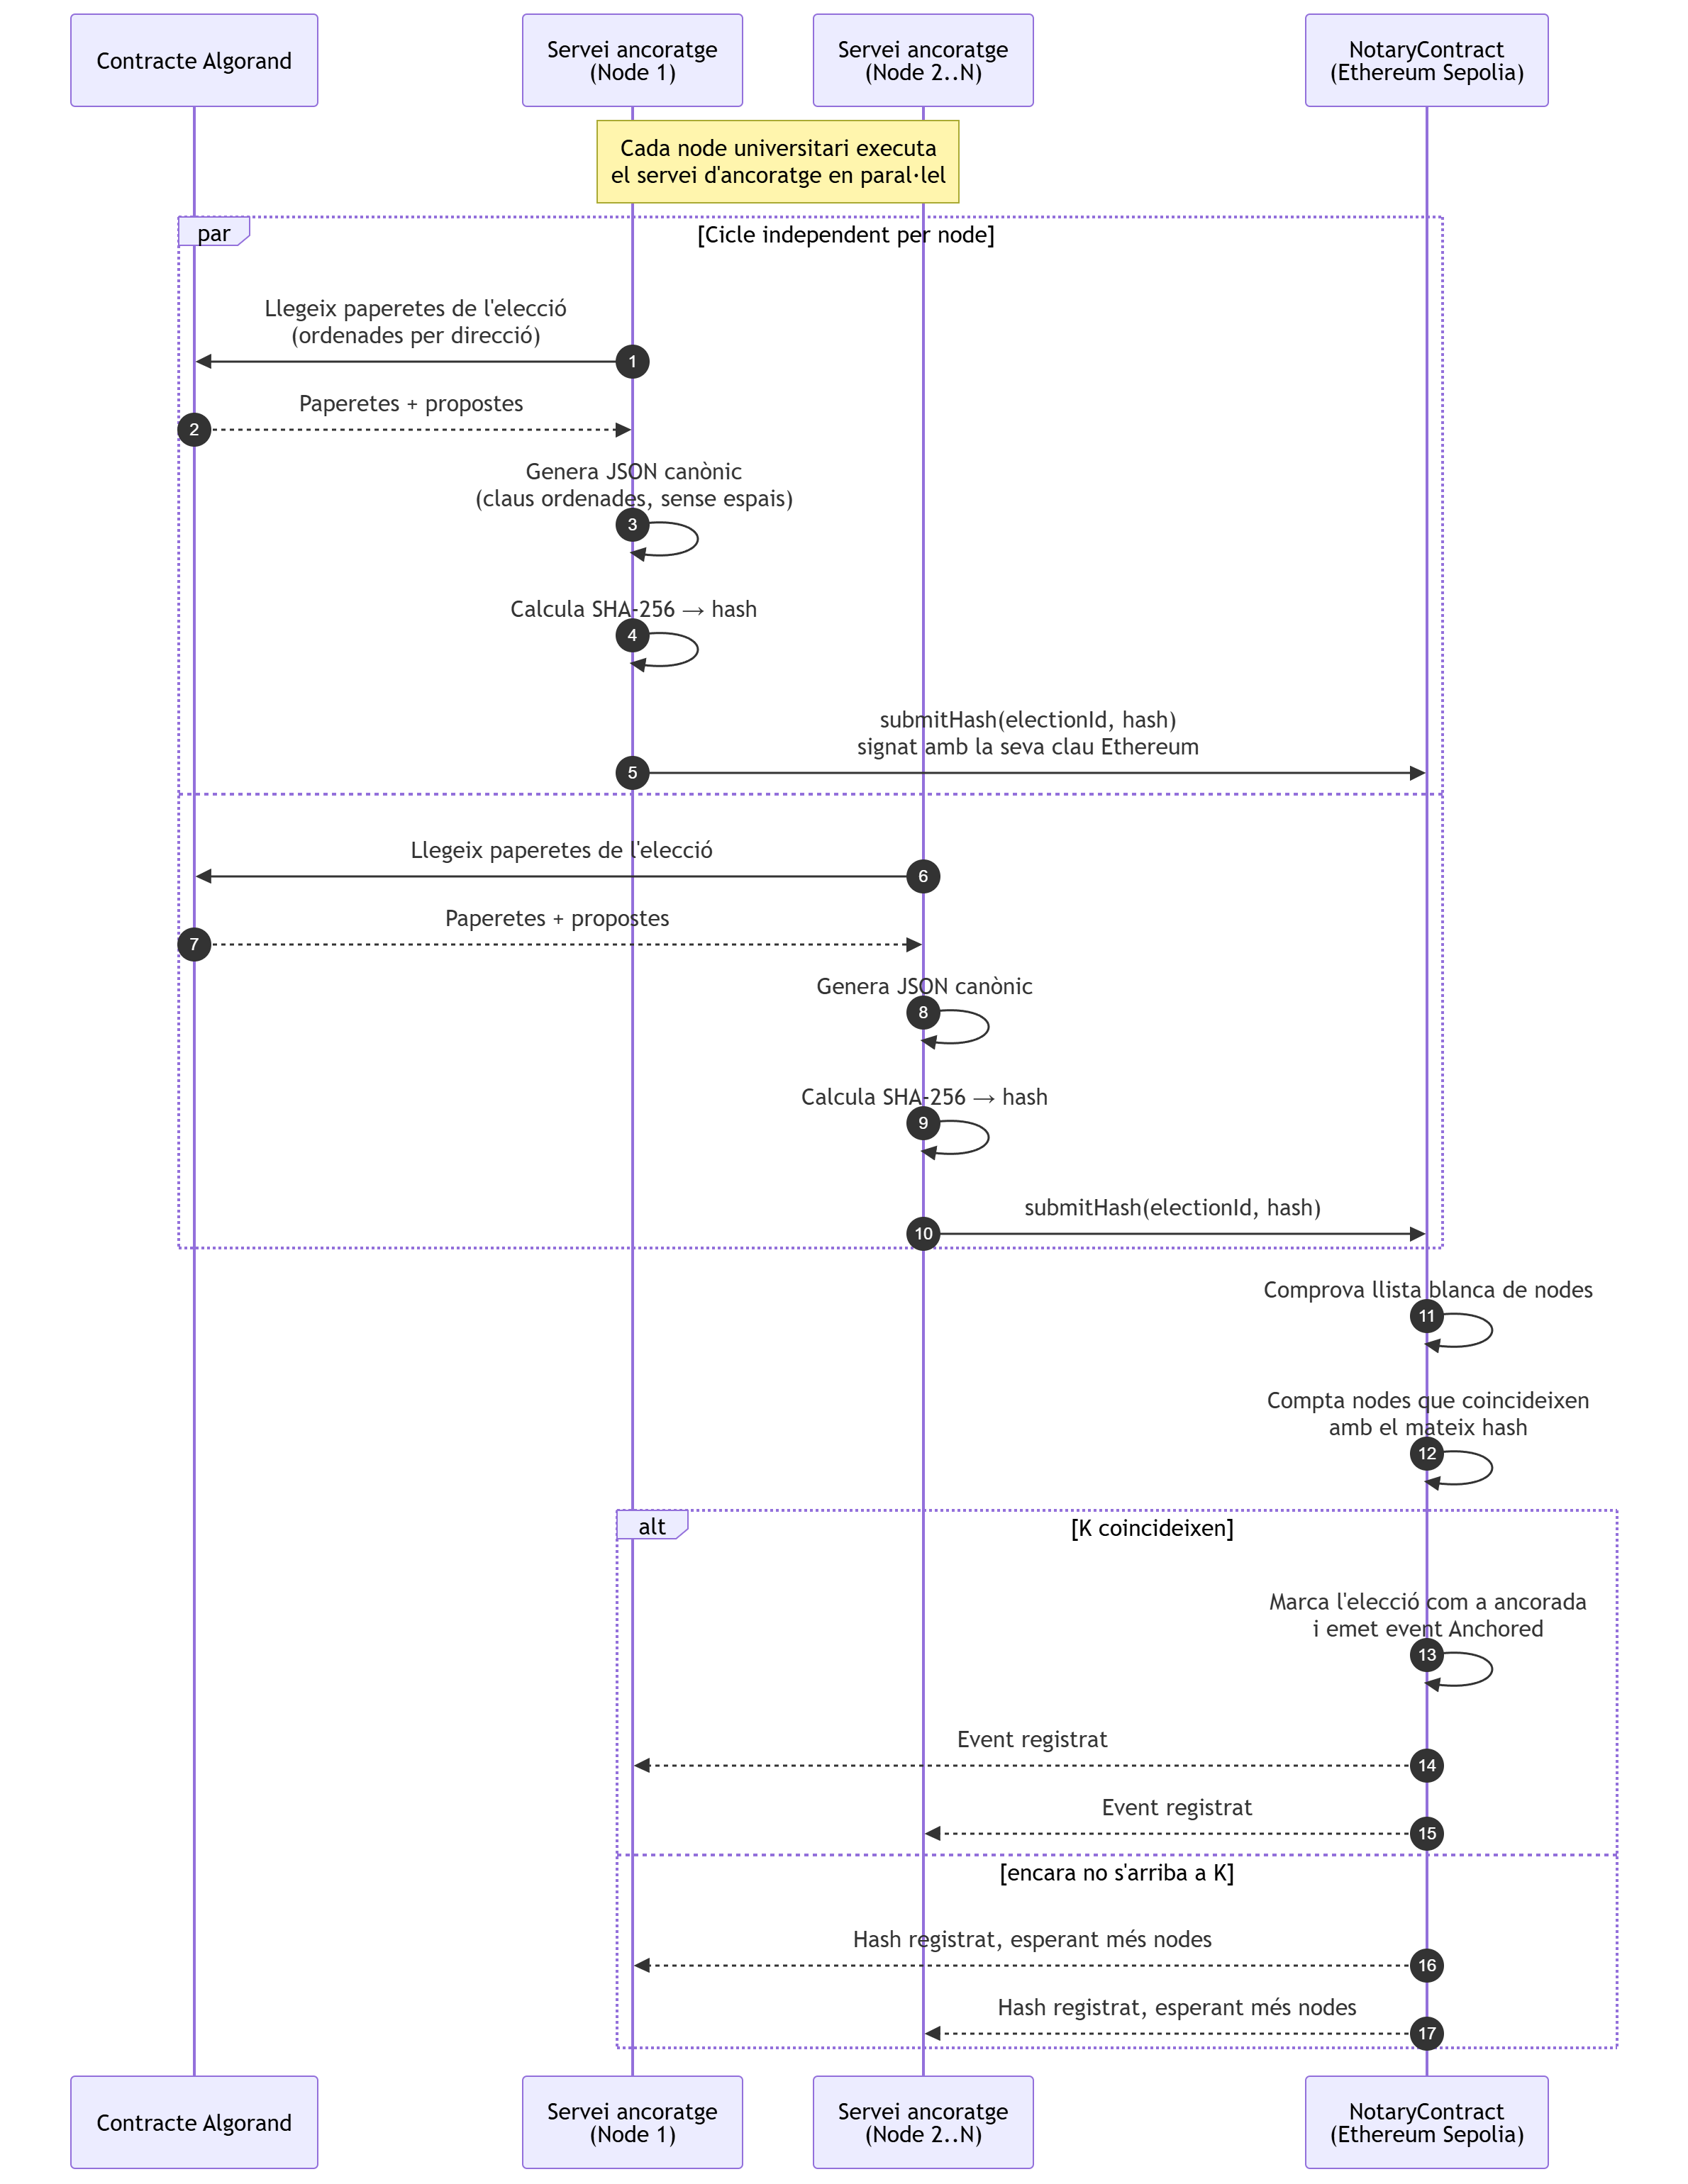
\includegraphics[width=\textwidth]{chapters/images/disseny/sequences/seq-anchoring}
    \caption{Diagrama de seqüència: ancoratge a Ethereum.}
    \label{fig:seq-anchoring}
\end{figure}

Aquest disseny garanteix dues propietats essencials.
Primer, que cap node individual pugui falsejar el resultat: necessita la coincidència de \textit{K-of-N}.
Segon, que el resultat sigui verificable sense necessitat de confiar en cap entitat central: qualsevol persona pot
consultar el contracte i comprovar quins nodes han signat, què han signat i quan.
